\documentclass[a4paper,11pt]{article}
\pagestyle{plain}
\usepackage{amsmath}
\usepackage{graphicx}
\begin{document}

\title{Assignment 2 - Differential Equations}
\date{July 22, 2012}
\author{Mohan S Nayaka}

\maketitle
1. Solve the differential equation
\[ x + y \frac{dy}{dx} = 0 \]
\emph{Answer}:
Separating the variables
\[ y \frac{dy}{dx} = -x \]
\[ ydy = -xdx \]
Integrating both sides, we obtain:
\[ \int y\,dy = \int -x\,dx \]
\[ \frac{y^2}{2} = -\frac{x^2}{2} + C_1 \]
\[ y^2 = -x^2 + 2 * C_1 \]
Thus, the solution is
{\renewcommand{\arraystretch}{1.5}
\begin{tabular}{|c|}
\hline
$x^2 + y^2 = C$ \\
\hline
\end{tabular}}
\begin{center}
where $C = 2 * C_1$.
\end{center}

\maketitle
2. Generate a family of curves for the above equation and find a particular solution for $y(0) = 10$.
\\
\emph{Answer}:
The family of curves is a set of circles with centre at the origin.\\
\newpage
%This is a very simple method of including an image (via TeX commands in circles.tex)
% \input was used instead of \include since the latter inroduces a page break
% which is not desirable.
%% GNUPLOT: LaTeX picture
\setlength{\unitlength}{0.240900pt}
\ifx\plotpoint\undefined\newsavebox{\plotpoint}\fi
\sbox{\plotpoint}{\rule[-0.200pt]{0.400pt}{0.400pt}}%
\begin{picture}(1500,900)(0,0)
\sbox{\plotpoint}{\rule[-0.200pt]{0.400pt}{0.400pt}}%
\put(508.0,131.0){\rule[-0.200pt]{145.504pt}{0.400pt}}
\put(508.0,131.0){\rule[-0.200pt]{4.818pt}{0.400pt}}
\put(488,131){\makebox(0,0)[r]{-20}}
\put(1092.0,131.0){\rule[-0.200pt]{4.818pt}{0.400pt}}
\put(508.0,207.0){\rule[-0.200pt]{145.504pt}{0.400pt}}
\put(508.0,207.0){\rule[-0.200pt]{4.818pt}{0.400pt}}
\put(488,207){\makebox(0,0)[r]{-15}}
\put(1092.0,207.0){\rule[-0.200pt]{4.818pt}{0.400pt}}
\put(508.0,282.0){\rule[-0.200pt]{145.504pt}{0.400pt}}
\put(508.0,282.0){\rule[-0.200pt]{4.818pt}{0.400pt}}
\put(488,282){\makebox(0,0)[r]{-10}}
\put(1092.0,282.0){\rule[-0.200pt]{4.818pt}{0.400pt}}
\put(508.0,358.0){\rule[-0.200pt]{145.504pt}{0.400pt}}
\put(508.0,358.0){\rule[-0.200pt]{4.818pt}{0.400pt}}
\put(488,358){\makebox(0,0)[r]{-5}}
\put(1092.0,358.0){\rule[-0.200pt]{4.818pt}{0.400pt}}
\put(508.0,433.0){\rule[-0.200pt]{145.504pt}{0.400pt}}
\put(508.0,433.0){\rule[-0.200pt]{4.818pt}{0.400pt}}
\put(488,433){\makebox(0,0)[r]{ 0}}
\put(1092.0,433.0){\rule[-0.200pt]{4.818pt}{0.400pt}}
\put(508.0,509.0){\rule[-0.200pt]{145.504pt}{0.400pt}}
\put(508.0,509.0){\rule[-0.200pt]{4.818pt}{0.400pt}}
\put(488,509){\makebox(0,0)[r]{ 5}}
\put(1092.0,509.0){\rule[-0.200pt]{4.818pt}{0.400pt}}
\put(508.0,584.0){\rule[-0.200pt]{145.504pt}{0.400pt}}
\put(508.0,584.0){\rule[-0.200pt]{4.818pt}{0.400pt}}
\put(488,584){\makebox(0,0)[r]{ 10}}
\put(1092.0,584.0){\rule[-0.200pt]{4.818pt}{0.400pt}}
\put(508.0,660.0){\rule[-0.200pt]{145.504pt}{0.400pt}}
\put(508.0,660.0){\rule[-0.200pt]{4.818pt}{0.400pt}}
\put(488,660){\makebox(0,0)[r]{ 15}}
\put(1092.0,660.0){\rule[-0.200pt]{4.818pt}{0.400pt}}
\put(508.0,735.0){\rule[-0.200pt]{145.504pt}{0.400pt}}
\put(508.0,735.0){\rule[-0.200pt]{4.818pt}{0.400pt}}
\put(488,735){\makebox(0,0)[r]{ 20}}
\put(1092.0,735.0){\rule[-0.200pt]{4.818pt}{0.400pt}}
\put(508.0,131.0){\rule[-0.200pt]{0.400pt}{145.504pt}}
\put(508.0,131.0){\rule[-0.200pt]{0.400pt}{4.818pt}}
\put(508,90){\makebox(0,0){-20}}
\put(508.0,715.0){\rule[-0.200pt]{0.400pt}{4.818pt}}
\put(584.0,131.0){\rule[-0.200pt]{0.400pt}{145.504pt}}
\put(584.0,131.0){\rule[-0.200pt]{0.400pt}{4.818pt}}
\put(584,90){\makebox(0,0){-15}}
\put(584.0,715.0){\rule[-0.200pt]{0.400pt}{4.818pt}}
\put(659.0,131.0){\rule[-0.200pt]{0.400pt}{145.504pt}}
\put(659.0,131.0){\rule[-0.200pt]{0.400pt}{4.818pt}}
\put(659,90){\makebox(0,0){-10}}
\put(659.0,715.0){\rule[-0.200pt]{0.400pt}{4.818pt}}
\put(735.0,131.0){\rule[-0.200pt]{0.400pt}{145.504pt}}
\put(735.0,131.0){\rule[-0.200pt]{0.400pt}{4.818pt}}
\put(735,90){\makebox(0,0){-5}}
\put(735.0,715.0){\rule[-0.200pt]{0.400pt}{4.818pt}}
\put(810.0,131.0){\rule[-0.200pt]{0.400pt}{145.504pt}}
\put(810.0,131.0){\rule[-0.200pt]{0.400pt}{4.818pt}}
\put(810,90){\makebox(0,0){ 0}}
\put(810.0,715.0){\rule[-0.200pt]{0.400pt}{4.818pt}}
\put(886.0,131.0){\rule[-0.200pt]{0.400pt}{145.504pt}}
\put(886.0,131.0){\rule[-0.200pt]{0.400pt}{4.818pt}}
\put(886,90){\makebox(0,0){ 5}}
\put(886.0,715.0){\rule[-0.200pt]{0.400pt}{4.818pt}}
\put(961.0,131.0){\rule[-0.200pt]{0.400pt}{145.504pt}}
\put(961.0,131.0){\rule[-0.200pt]{0.400pt}{4.818pt}}
\put(961,90){\makebox(0,0){ 10}}
\put(961.0,715.0){\rule[-0.200pt]{0.400pt}{4.818pt}}
\put(1037.0,131.0){\rule[-0.200pt]{0.400pt}{145.504pt}}
\put(1037.0,131.0){\rule[-0.200pt]{0.400pt}{4.818pt}}
\put(1037,90){\makebox(0,0){ 15}}
\put(1037.0,715.0){\rule[-0.200pt]{0.400pt}{4.818pt}}
\put(1112.0,131.0){\rule[-0.200pt]{0.400pt}{145.504pt}}
\put(1112.0,131.0){\rule[-0.200pt]{0.400pt}{4.818pt}}
\put(1112,90){\makebox(0,0){ 20}}
\put(1112.0,715.0){\rule[-0.200pt]{0.400pt}{4.818pt}}
\put(508.0,131.0){\rule[-0.200pt]{0.400pt}{145.504pt}}
\put(508.0,131.0){\rule[-0.200pt]{145.504pt}{0.400pt}}
\put(1112.0,131.0){\rule[-0.200pt]{0.400pt}{145.504pt}}
\put(508.0,735.0){\rule[-0.200pt]{145.504pt}{0.400pt}}
\put(387,433){\makebox(0,0){y}}
\put(810,29){\makebox(0,0){x}}
\put(810,838){\makebox(0,0){Family of curves (circles) satisfying the differential equation}}
\put(810,797){\makebox(0,0){Circles are of radii 4,8,10,15 and 19 units}}
\put(810,493){\usebox{\plotpoint}}
\put(818,491.67){\rule{0.723pt}{0.400pt}}
\multiput(818.00,492.17)(1.500,-1.000){2}{\rule{0.361pt}{0.400pt}}
\put(821,490.67){\rule{0.964pt}{0.400pt}}
\multiput(821.00,491.17)(2.000,-1.000){2}{\rule{0.482pt}{0.400pt}}
\put(825,489.67){\rule{0.964pt}{0.400pt}}
\multiput(825.00,490.17)(2.000,-1.000){2}{\rule{0.482pt}{0.400pt}}
\put(829,488.67){\rule{0.723pt}{0.400pt}}
\multiput(829.00,489.17)(1.500,-1.000){2}{\rule{0.361pt}{0.400pt}}
\put(832,487.67){\rule{0.964pt}{0.400pt}}
\multiput(832.00,488.17)(2.000,-1.000){2}{\rule{0.482pt}{0.400pt}}
\put(836,486.17){\rule{0.700pt}{0.400pt}}
\multiput(836.00,487.17)(1.547,-2.000){2}{\rule{0.350pt}{0.400pt}}
\put(839,484.17){\rule{0.900pt}{0.400pt}}
\multiput(839.00,485.17)(2.132,-2.000){2}{\rule{0.450pt}{0.400pt}}
\put(843,482.17){\rule{0.700pt}{0.400pt}}
\multiput(843.00,483.17)(1.547,-2.000){2}{\rule{0.350pt}{0.400pt}}
\multiput(846.00,480.95)(0.462,-0.447){3}{\rule{0.500pt}{0.108pt}}
\multiput(846.00,481.17)(1.962,-3.000){2}{\rule{0.250pt}{0.400pt}}
\put(849,477.17){\rule{0.700pt}{0.400pt}}
\multiput(849.00,478.17)(1.547,-2.000){2}{\rule{0.350pt}{0.400pt}}
\put(852.17,474){\rule{0.400pt}{0.700pt}}
\multiput(851.17,475.55)(2.000,-1.547){2}{\rule{0.400pt}{0.350pt}}
\multiput(854.00,472.95)(0.462,-0.447){3}{\rule{0.500pt}{0.108pt}}
\multiput(854.00,473.17)(1.962,-3.000){2}{\rule{0.250pt}{0.400pt}}
\put(857.17,468){\rule{0.400pt}{0.700pt}}
\multiput(856.17,469.55)(2.000,-1.547){2}{\rule{0.400pt}{0.350pt}}
\put(859.17,465){\rule{0.400pt}{0.700pt}}
\multiput(858.17,466.55)(2.000,-1.547){2}{\rule{0.400pt}{0.350pt}}
\put(861.17,462){\rule{0.400pt}{0.700pt}}
\multiput(860.17,463.55)(2.000,-1.547){2}{\rule{0.400pt}{0.350pt}}
\put(863.17,458){\rule{0.400pt}{0.900pt}}
\multiput(862.17,460.13)(2.000,-2.132){2}{\rule{0.400pt}{0.450pt}}
\put(864.67,455){\rule{0.400pt}{0.723pt}}
\multiput(864.17,456.50)(1.000,-1.500){2}{\rule{0.400pt}{0.361pt}}
\put(866.17,451){\rule{0.400pt}{0.900pt}}
\multiput(865.17,453.13)(2.000,-2.132){2}{\rule{0.400pt}{0.450pt}}
\put(867.67,447){\rule{0.400pt}{0.964pt}}
\multiput(867.17,449.00)(1.000,-2.000){2}{\rule{0.400pt}{0.482pt}}
\put(810.0,493.0){\rule[-0.200pt]{1.927pt}{0.400pt}}
\put(868.67,440){\rule{0.400pt}{0.723pt}}
\multiput(868.17,441.50)(1.000,-1.500){2}{\rule{0.400pt}{0.361pt}}
\put(869.0,443.0){\rule[-0.200pt]{0.400pt}{0.964pt}}
\put(868.67,421){\rule{0.400pt}{0.723pt}}
\multiput(869.17,422.50)(-1.000,-1.500){2}{\rule{0.400pt}{0.361pt}}
\put(867.67,417){\rule{0.400pt}{0.964pt}}
\multiput(868.17,419.00)(-1.000,-2.000){2}{\rule{0.400pt}{0.482pt}}
\put(866.67,413){\rule{0.400pt}{0.964pt}}
\multiput(867.17,415.00)(-1.000,-2.000){2}{\rule{0.400pt}{0.482pt}}
\put(865.67,410){\rule{0.400pt}{0.723pt}}
\multiput(866.17,411.50)(-1.000,-1.500){2}{\rule{0.400pt}{0.361pt}}
\put(864.17,406){\rule{0.400pt}{0.900pt}}
\multiput(865.17,408.13)(-2.000,-2.132){2}{\rule{0.400pt}{0.450pt}}
\put(862.17,403){\rule{0.400pt}{0.700pt}}
\multiput(863.17,404.55)(-2.000,-1.547){2}{\rule{0.400pt}{0.350pt}}
\put(860.17,400){\rule{0.400pt}{0.700pt}}
\multiput(861.17,401.55)(-2.000,-1.547){2}{\rule{0.400pt}{0.350pt}}
\put(858.17,396){\rule{0.400pt}{0.900pt}}
\multiput(859.17,398.13)(-2.000,-2.132){2}{\rule{0.400pt}{0.450pt}}
\put(856.17,393){\rule{0.400pt}{0.700pt}}
\multiput(857.17,394.55)(-2.000,-1.547){2}{\rule{0.400pt}{0.350pt}}
\put(853,391.17){\rule{0.700pt}{0.400pt}}
\multiput(854.55,392.17)(-1.547,-2.000){2}{\rule{0.350pt}{0.400pt}}
\multiput(850.92,389.95)(-0.462,-0.447){3}{\rule{0.500pt}{0.108pt}}
\multiput(851.96,390.17)(-1.962,-3.000){2}{\rule{0.250pt}{0.400pt}}
\put(847,386.17){\rule{0.700pt}{0.400pt}}
\multiput(848.55,387.17)(-1.547,-2.000){2}{\rule{0.350pt}{0.400pt}}
\multiput(844.92,384.95)(-0.462,-0.447){3}{\rule{0.500pt}{0.108pt}}
\multiput(845.96,385.17)(-1.962,-3.000){2}{\rule{0.250pt}{0.400pt}}
\put(841,381.17){\rule{0.700pt}{0.400pt}}
\multiput(842.55,382.17)(-1.547,-2.000){2}{\rule{0.350pt}{0.400pt}}
\put(838,379.17){\rule{0.700pt}{0.400pt}}
\multiput(839.55,380.17)(-1.547,-2.000){2}{\rule{0.350pt}{0.400pt}}
\put(834,377.67){\rule{0.964pt}{0.400pt}}
\multiput(836.00,378.17)(-2.000,-1.000){2}{\rule{0.482pt}{0.400pt}}
\put(831,376.17){\rule{0.700pt}{0.400pt}}
\multiput(832.55,377.17)(-1.547,-2.000){2}{\rule{0.350pt}{0.400pt}}
\put(827,374.67){\rule{0.964pt}{0.400pt}}
\multiput(829.00,375.17)(-2.000,-1.000){2}{\rule{0.482pt}{0.400pt}}
\put(823,373.67){\rule{0.964pt}{0.400pt}}
\multiput(825.00,374.17)(-2.000,-1.000){2}{\rule{0.482pt}{0.400pt}}
\put(820,372.67){\rule{0.723pt}{0.400pt}}
\multiput(821.50,373.17)(-1.500,-1.000){2}{\rule{0.361pt}{0.400pt}}
\put(870.0,424.0){\rule[-0.200pt]{0.400pt}{3.854pt}}
\put(797,372.67){\rule{0.723pt}{0.400pt}}
\multiput(798.50,372.17)(-1.500,1.000){2}{\rule{0.361pt}{0.400pt}}
\put(793,373.67){\rule{0.964pt}{0.400pt}}
\multiput(795.00,373.17)(-2.000,1.000){2}{\rule{0.482pt}{0.400pt}}
\put(789,374.67){\rule{0.964pt}{0.400pt}}
\multiput(791.00,374.17)(-2.000,1.000){2}{\rule{0.482pt}{0.400pt}}
\put(786,376.17){\rule{0.700pt}{0.400pt}}
\multiput(787.55,375.17)(-1.547,2.000){2}{\rule{0.350pt}{0.400pt}}
\put(782,377.67){\rule{0.964pt}{0.400pt}}
\multiput(784.00,377.17)(-2.000,1.000){2}{\rule{0.482pt}{0.400pt}}
\put(779,379.17){\rule{0.700pt}{0.400pt}}
\multiput(780.55,378.17)(-1.547,2.000){2}{\rule{0.350pt}{0.400pt}}
\put(776,381.17){\rule{0.700pt}{0.400pt}}
\multiput(777.55,380.17)(-1.547,2.000){2}{\rule{0.350pt}{0.400pt}}
\multiput(773.92,383.61)(-0.462,0.447){3}{\rule{0.500pt}{0.108pt}}
\multiput(774.96,382.17)(-1.962,3.000){2}{\rule{0.250pt}{0.400pt}}
\put(770,386.17){\rule{0.700pt}{0.400pt}}
\multiput(771.55,385.17)(-1.547,2.000){2}{\rule{0.350pt}{0.400pt}}
\multiput(767.92,388.61)(-0.462,0.447){3}{\rule{0.500pt}{0.108pt}}
\multiput(768.96,387.17)(-1.962,3.000){2}{\rule{0.250pt}{0.400pt}}
\put(764,391.17){\rule{0.700pt}{0.400pt}}
\multiput(765.55,390.17)(-1.547,2.000){2}{\rule{0.350pt}{0.400pt}}
\put(762.17,393){\rule{0.400pt}{0.700pt}}
\multiput(763.17,393.00)(-2.000,1.547){2}{\rule{0.400pt}{0.350pt}}
\put(760.17,396){\rule{0.400pt}{0.900pt}}
\multiput(761.17,396.00)(-2.000,2.132){2}{\rule{0.400pt}{0.450pt}}
\put(758.17,400){\rule{0.400pt}{0.700pt}}
\multiput(759.17,400.00)(-2.000,1.547){2}{\rule{0.400pt}{0.350pt}}
\put(756.17,403){\rule{0.400pt}{0.700pt}}
\multiput(757.17,403.00)(-2.000,1.547){2}{\rule{0.400pt}{0.350pt}}
\put(754.17,406){\rule{0.400pt}{0.900pt}}
\multiput(755.17,406.00)(-2.000,2.132){2}{\rule{0.400pt}{0.450pt}}
\put(752.67,410){\rule{0.400pt}{0.723pt}}
\multiput(753.17,410.00)(-1.000,1.500){2}{\rule{0.400pt}{0.361pt}}
\put(751.67,413){\rule{0.400pt}{0.964pt}}
\multiput(752.17,413.00)(-1.000,2.000){2}{\rule{0.400pt}{0.482pt}}
\put(750.67,417){\rule{0.400pt}{0.964pt}}
\multiput(751.17,417.00)(-1.000,2.000){2}{\rule{0.400pt}{0.482pt}}
\put(749.67,421){\rule{0.400pt}{0.723pt}}
\multiput(750.17,421.00)(-1.000,1.500){2}{\rule{0.400pt}{0.361pt}}
\put(800.0,373.0){\rule[-0.200pt]{4.818pt}{0.400pt}}
\put(749.67,440){\rule{0.400pt}{0.723pt}}
\multiput(749.17,440.00)(1.000,1.500){2}{\rule{0.400pt}{0.361pt}}
\put(750.0,424.0){\rule[-0.200pt]{0.400pt}{3.854pt}}
\put(750.67,447){\rule{0.400pt}{0.964pt}}
\multiput(750.17,447.00)(1.000,2.000){2}{\rule{0.400pt}{0.482pt}}
\put(752.17,451){\rule{0.400pt}{0.900pt}}
\multiput(751.17,451.00)(2.000,2.132){2}{\rule{0.400pt}{0.450pt}}
\put(753.67,455){\rule{0.400pt}{0.723pt}}
\multiput(753.17,455.00)(1.000,1.500){2}{\rule{0.400pt}{0.361pt}}
\put(755.17,458){\rule{0.400pt}{0.900pt}}
\multiput(754.17,458.00)(2.000,2.132){2}{\rule{0.400pt}{0.450pt}}
\put(757.17,462){\rule{0.400pt}{0.700pt}}
\multiput(756.17,462.00)(2.000,1.547){2}{\rule{0.400pt}{0.350pt}}
\put(759.17,465){\rule{0.400pt}{0.700pt}}
\multiput(758.17,465.00)(2.000,1.547){2}{\rule{0.400pt}{0.350pt}}
\put(761.17,468){\rule{0.400pt}{0.700pt}}
\multiput(760.17,468.00)(2.000,1.547){2}{\rule{0.400pt}{0.350pt}}
\multiput(763.00,471.61)(0.462,0.447){3}{\rule{0.500pt}{0.108pt}}
\multiput(763.00,470.17)(1.962,3.000){2}{\rule{0.250pt}{0.400pt}}
\put(766.17,474){\rule{0.400pt}{0.700pt}}
\multiput(765.17,474.00)(2.000,1.547){2}{\rule{0.400pt}{0.350pt}}
\put(768,477.17){\rule{0.700pt}{0.400pt}}
\multiput(768.00,476.17)(1.547,2.000){2}{\rule{0.350pt}{0.400pt}}
\multiput(771.00,479.61)(0.462,0.447){3}{\rule{0.500pt}{0.108pt}}
\multiput(771.00,478.17)(1.962,3.000){2}{\rule{0.250pt}{0.400pt}}
\put(774,482.17){\rule{0.700pt}{0.400pt}}
\multiput(774.00,481.17)(1.547,2.000){2}{\rule{0.350pt}{0.400pt}}
\put(777,484.17){\rule{0.900pt}{0.400pt}}
\multiput(777.00,483.17)(2.132,2.000){2}{\rule{0.450pt}{0.400pt}}
\put(781,486.17){\rule{0.700pt}{0.400pt}}
\multiput(781.00,485.17)(1.547,2.000){2}{\rule{0.350pt}{0.400pt}}
\put(784,487.67){\rule{0.964pt}{0.400pt}}
\multiput(784.00,487.17)(2.000,1.000){2}{\rule{0.482pt}{0.400pt}}
\put(788,488.67){\rule{0.723pt}{0.400pt}}
\multiput(788.00,488.17)(1.500,1.000){2}{\rule{0.361pt}{0.400pt}}
\put(791,489.67){\rule{0.964pt}{0.400pt}}
\multiput(791.00,489.17)(2.000,1.000){2}{\rule{0.482pt}{0.400pt}}
\put(795,490.67){\rule{0.964pt}{0.400pt}}
\multiput(795.00,490.17)(2.000,1.000){2}{\rule{0.482pt}{0.400pt}}
\put(799,491.67){\rule{0.723pt}{0.400pt}}
\multiput(799.00,491.17)(1.500,1.000){2}{\rule{0.361pt}{0.400pt}}
\put(751.0,443.0){\rule[-0.200pt]{0.400pt}{0.964pt}}
\put(802.0,493.0){\rule[-0.200pt]{1.927pt}{0.400pt}}
\put(508.0,131.0){\rule[-0.200pt]{0.400pt}{145.504pt}}
\put(508.0,131.0){\rule[-0.200pt]{145.504pt}{0.400pt}}
\put(1112.0,131.0){\rule[-0.200pt]{0.400pt}{145.504pt}}
\put(508.0,735.0){\rule[-0.200pt]{145.504pt}{0.400pt}}
\put(508.0,131.0){\rule[-0.200pt]{145.504pt}{0.400pt}}
\put(508.0,131.0){\rule[-0.200pt]{4.818pt}{0.400pt}}
\put(488,131){\makebox(0,0)[r]{-20}}
\put(1092.0,131.0){\rule[-0.200pt]{4.818pt}{0.400pt}}
\put(508.0,207.0){\rule[-0.200pt]{145.504pt}{0.400pt}}
\put(508.0,207.0){\rule[-0.200pt]{4.818pt}{0.400pt}}
\put(488,207){\makebox(0,0)[r]{-15}}
\put(1092.0,207.0){\rule[-0.200pt]{4.818pt}{0.400pt}}
\put(508.0,282.0){\rule[-0.200pt]{145.504pt}{0.400pt}}
\put(508.0,282.0){\rule[-0.200pt]{4.818pt}{0.400pt}}
\put(488,282){\makebox(0,0)[r]{-10}}
\put(1092.0,282.0){\rule[-0.200pt]{4.818pt}{0.400pt}}
\put(508.0,358.0){\rule[-0.200pt]{145.504pt}{0.400pt}}
\put(508.0,358.0){\rule[-0.200pt]{4.818pt}{0.400pt}}
\put(488,358){\makebox(0,0)[r]{-5}}
\put(1092.0,358.0){\rule[-0.200pt]{4.818pt}{0.400pt}}
\put(508.0,433.0){\rule[-0.200pt]{145.504pt}{0.400pt}}
\put(508.0,433.0){\rule[-0.200pt]{4.818pt}{0.400pt}}
\put(488,433){\makebox(0,0)[r]{ 0}}
\put(1092.0,433.0){\rule[-0.200pt]{4.818pt}{0.400pt}}
\put(508.0,509.0){\rule[-0.200pt]{145.504pt}{0.400pt}}
\put(508.0,509.0){\rule[-0.200pt]{4.818pt}{0.400pt}}
\put(488,509){\makebox(0,0)[r]{ 5}}
\put(1092.0,509.0){\rule[-0.200pt]{4.818pt}{0.400pt}}
\put(508.0,584.0){\rule[-0.200pt]{145.504pt}{0.400pt}}
\put(508.0,584.0){\rule[-0.200pt]{4.818pt}{0.400pt}}
\put(488,584){\makebox(0,0)[r]{ 10}}
\put(1092.0,584.0){\rule[-0.200pt]{4.818pt}{0.400pt}}
\put(508.0,660.0){\rule[-0.200pt]{145.504pt}{0.400pt}}
\put(508.0,660.0){\rule[-0.200pt]{4.818pt}{0.400pt}}
\put(488,660){\makebox(0,0)[r]{ 15}}
\put(1092.0,660.0){\rule[-0.200pt]{4.818pt}{0.400pt}}
\put(508.0,735.0){\rule[-0.200pt]{145.504pt}{0.400pt}}
\put(508.0,735.0){\rule[-0.200pt]{4.818pt}{0.400pt}}
\put(488,735){\makebox(0,0)[r]{ 20}}
\put(1092.0,735.0){\rule[-0.200pt]{4.818pt}{0.400pt}}
\put(508.0,131.0){\rule[-0.200pt]{0.400pt}{145.504pt}}
\put(508.0,131.0){\rule[-0.200pt]{0.400pt}{4.818pt}}
\put(508,90){\makebox(0,0){-20}}
\put(508.0,715.0){\rule[-0.200pt]{0.400pt}{4.818pt}}
\put(584.0,131.0){\rule[-0.200pt]{0.400pt}{145.504pt}}
\put(584.0,131.0){\rule[-0.200pt]{0.400pt}{4.818pt}}
\put(584,90){\makebox(0,0){-15}}
\put(584.0,715.0){\rule[-0.200pt]{0.400pt}{4.818pt}}
\put(659.0,131.0){\rule[-0.200pt]{0.400pt}{145.504pt}}
\put(659.0,131.0){\rule[-0.200pt]{0.400pt}{4.818pt}}
\put(659,90){\makebox(0,0){-10}}
\put(659.0,715.0){\rule[-0.200pt]{0.400pt}{4.818pt}}
\put(735.0,131.0){\rule[-0.200pt]{0.400pt}{145.504pt}}
\put(735.0,131.0){\rule[-0.200pt]{0.400pt}{4.818pt}}
\put(735,90){\makebox(0,0){-5}}
\put(735.0,715.0){\rule[-0.200pt]{0.400pt}{4.818pt}}
\put(810.0,131.0){\rule[-0.200pt]{0.400pt}{145.504pt}}
\put(810.0,131.0){\rule[-0.200pt]{0.400pt}{4.818pt}}
\put(810,90){\makebox(0,0){ 0}}
\put(810.0,715.0){\rule[-0.200pt]{0.400pt}{4.818pt}}
\put(886.0,131.0){\rule[-0.200pt]{0.400pt}{145.504pt}}
\put(886.0,131.0){\rule[-0.200pt]{0.400pt}{4.818pt}}
\put(886,90){\makebox(0,0){ 5}}
\put(886.0,715.0){\rule[-0.200pt]{0.400pt}{4.818pt}}
\put(961.0,131.0){\rule[-0.200pt]{0.400pt}{145.504pt}}
\put(961.0,131.0){\rule[-0.200pt]{0.400pt}{4.818pt}}
\put(961,90){\makebox(0,0){ 10}}
\put(961.0,715.0){\rule[-0.200pt]{0.400pt}{4.818pt}}
\put(1037.0,131.0){\rule[-0.200pt]{0.400pt}{145.504pt}}
\put(1037.0,131.0){\rule[-0.200pt]{0.400pt}{4.818pt}}
\put(1037,90){\makebox(0,0){ 15}}
\put(1037.0,715.0){\rule[-0.200pt]{0.400pt}{4.818pt}}
\put(1112.0,131.0){\rule[-0.200pt]{0.400pt}{145.504pt}}
\put(1112.0,131.0){\rule[-0.200pt]{0.400pt}{4.818pt}}
\put(1112,90){\makebox(0,0){ 20}}
\put(1112.0,715.0){\rule[-0.200pt]{0.400pt}{4.818pt}}
\put(508.0,131.0){\rule[-0.200pt]{0.400pt}{145.504pt}}
\put(508.0,131.0){\rule[-0.200pt]{145.504pt}{0.400pt}}
\put(1112.0,131.0){\rule[-0.200pt]{0.400pt}{145.504pt}}
\put(508.0,735.0){\rule[-0.200pt]{145.504pt}{0.400pt}}
\put(387,433){\makebox(0,0){y}}
\put(810,29){\makebox(0,0){x}}
\put(810,838){\makebox(0,0){Family of curves (circles) satisfying the differential equation}}
\put(810,797){\makebox(0,0){Circles are of radii 4,8,10,15 and 19 units}}
\put(810,554){\usebox{\plotpoint}}
\put(818,552.67){\rule{1.686pt}{0.400pt}}
\multiput(818.00,553.17)(3.500,-1.000){2}{\rule{0.843pt}{0.400pt}}
\put(825,551.67){\rule{1.927pt}{0.400pt}}
\multiput(825.00,552.17)(4.000,-1.000){2}{\rule{0.964pt}{0.400pt}}
\put(833,550.17){\rule{1.500pt}{0.400pt}}
\multiput(833.00,551.17)(3.887,-2.000){2}{\rule{0.750pt}{0.400pt}}
\put(840,548.17){\rule{1.700pt}{0.400pt}}
\multiput(840.00,549.17)(4.472,-2.000){2}{\rule{0.850pt}{0.400pt}}
\multiput(848.00,546.95)(1.355,-0.447){3}{\rule{1.033pt}{0.108pt}}
\multiput(848.00,547.17)(4.855,-3.000){2}{\rule{0.517pt}{0.400pt}}
\multiput(855.00,543.95)(1.355,-0.447){3}{\rule{1.033pt}{0.108pt}}
\multiput(855.00,544.17)(4.855,-3.000){2}{\rule{0.517pt}{0.400pt}}
\multiput(862.00,540.95)(1.355,-0.447){3}{\rule{1.033pt}{0.108pt}}
\multiput(862.00,541.17)(4.855,-3.000){2}{\rule{0.517pt}{0.400pt}}
\multiput(869.00,537.94)(0.774,-0.468){5}{\rule{0.700pt}{0.113pt}}
\multiput(869.00,538.17)(4.547,-4.000){2}{\rule{0.350pt}{0.400pt}}
\multiput(875.00,533.93)(0.710,-0.477){7}{\rule{0.660pt}{0.115pt}}
\multiput(875.00,534.17)(5.630,-5.000){2}{\rule{0.330pt}{0.400pt}}
\multiput(882.00,528.94)(0.774,-0.468){5}{\rule{0.700pt}{0.113pt}}
\multiput(882.00,529.17)(4.547,-4.000){2}{\rule{0.350pt}{0.400pt}}
\multiput(888.59,523.59)(0.477,-0.599){7}{\rule{0.115pt}{0.580pt}}
\multiput(887.17,524.80)(5.000,-4.796){2}{\rule{0.400pt}{0.290pt}}
\multiput(893.00,518.93)(0.599,-0.477){7}{\rule{0.580pt}{0.115pt}}
\multiput(893.00,519.17)(4.796,-5.000){2}{\rule{0.290pt}{0.400pt}}
\multiput(899.59,512.59)(0.477,-0.599){7}{\rule{0.115pt}{0.580pt}}
\multiput(898.17,513.80)(5.000,-4.796){2}{\rule{0.400pt}{0.290pt}}
\multiput(904.60,506.09)(0.468,-0.774){5}{\rule{0.113pt}{0.700pt}}
\multiput(903.17,507.55)(4.000,-4.547){2}{\rule{0.400pt}{0.350pt}}
\multiput(908.59,500.59)(0.477,-0.599){7}{\rule{0.115pt}{0.580pt}}
\multiput(907.17,501.80)(5.000,-4.796){2}{\rule{0.400pt}{0.290pt}}
\multiput(913.61,492.71)(0.447,-1.355){3}{\rule{0.108pt}{1.033pt}}
\multiput(912.17,494.86)(3.000,-4.855){2}{\rule{0.400pt}{0.517pt}}
\multiput(916.60,486.68)(0.468,-0.920){5}{\rule{0.113pt}{0.800pt}}
\multiput(915.17,488.34)(4.000,-5.340){2}{\rule{0.400pt}{0.400pt}}
\multiput(920.61,478.71)(0.447,-1.355){3}{\rule{0.108pt}{1.033pt}}
\multiput(919.17,480.86)(3.000,-4.855){2}{\rule{0.400pt}{0.517pt}}
\put(923.17,469){\rule{0.400pt}{1.500pt}}
\multiput(922.17,472.89)(2.000,-3.887){2}{\rule{0.400pt}{0.750pt}}
\put(925.17,461){\rule{0.400pt}{1.700pt}}
\multiput(924.17,465.47)(2.000,-4.472){2}{\rule{0.400pt}{0.850pt}}
\put(927.17,454){\rule{0.400pt}{1.500pt}}
\multiput(926.17,457.89)(2.000,-3.887){2}{\rule{0.400pt}{0.750pt}}
\put(928.67,446){\rule{0.400pt}{1.927pt}}
\multiput(928.17,450.00)(1.000,-4.000){2}{\rule{0.400pt}{0.964pt}}
\put(929.67,439){\rule{0.400pt}{1.686pt}}
\multiput(929.17,442.50)(1.000,-3.500){2}{\rule{0.400pt}{0.843pt}}
\put(810.0,554.0){\rule[-0.200pt]{1.927pt}{0.400pt}}
\put(929.67,423){\rule{0.400pt}{1.927pt}}
\multiput(930.17,427.00)(-1.000,-4.000){2}{\rule{0.400pt}{0.964pt}}
\put(931.0,431.0){\rule[-0.200pt]{0.400pt}{1.927pt}}
\put(928.17,408){\rule{0.400pt}{1.700pt}}
\multiput(929.17,412.47)(-2.000,-4.472){2}{\rule{0.400pt}{0.850pt}}
\put(926.17,401){\rule{0.400pt}{1.500pt}}
\multiput(927.17,404.89)(-2.000,-3.887){2}{\rule{0.400pt}{0.750pt}}
\put(924.17,393){\rule{0.400pt}{1.700pt}}
\multiput(925.17,397.47)(-2.000,-4.472){2}{\rule{0.400pt}{0.850pt}}
\multiput(922.95,388.71)(-0.447,-1.355){3}{\rule{0.108pt}{1.033pt}}
\multiput(923.17,390.86)(-3.000,-4.855){2}{\rule{0.400pt}{0.517pt}}
\multiput(919.95,381.71)(-0.447,-1.355){3}{\rule{0.108pt}{1.033pt}}
\multiput(920.17,383.86)(-3.000,-4.855){2}{\rule{0.400pt}{0.517pt}}
\multiput(916.95,375.26)(-0.447,-1.132){3}{\rule{0.108pt}{0.900pt}}
\multiput(917.17,377.13)(-3.000,-4.132){2}{\rule{0.400pt}{0.450pt}}
\multiput(913.94,369.68)(-0.468,-0.920){5}{\rule{0.113pt}{0.800pt}}
\multiput(914.17,371.34)(-4.000,-5.340){2}{\rule{0.400pt}{0.400pt}}
\multiput(909.93,363.59)(-0.477,-0.599){7}{\rule{0.115pt}{0.580pt}}
\multiput(910.17,364.80)(-5.000,-4.796){2}{\rule{0.400pt}{0.290pt}}
\multiput(904.93,357.59)(-0.477,-0.599){7}{\rule{0.115pt}{0.580pt}}
\multiput(905.17,358.80)(-5.000,-4.796){2}{\rule{0.400pt}{0.290pt}}
\multiput(899.93,351.59)(-0.477,-0.599){7}{\rule{0.115pt}{0.580pt}}
\multiput(900.17,352.80)(-5.000,-4.796){2}{\rule{0.400pt}{0.290pt}}
\multiput(893.92,346.93)(-0.487,-0.477){7}{\rule{0.500pt}{0.115pt}}
\multiput(894.96,347.17)(-3.962,-5.000){2}{\rule{0.250pt}{0.400pt}}
\multiput(888.59,341.93)(-0.599,-0.477){7}{\rule{0.580pt}{0.115pt}}
\multiput(889.80,342.17)(-4.796,-5.000){2}{\rule{0.290pt}{0.400pt}}
\multiput(882.59,336.93)(-0.599,-0.477){7}{\rule{0.580pt}{0.115pt}}
\multiput(883.80,337.17)(-4.796,-5.000){2}{\rule{0.290pt}{0.400pt}}
\multiput(875.68,331.94)(-0.920,-0.468){5}{\rule{0.800pt}{0.113pt}}
\multiput(877.34,332.17)(-5.340,-4.000){2}{\rule{0.400pt}{0.400pt}}
\multiput(867.71,327.95)(-1.355,-0.447){3}{\rule{1.033pt}{0.108pt}}
\multiput(869.86,328.17)(-4.855,-3.000){2}{\rule{0.517pt}{0.400pt}}
\multiput(861.68,324.94)(-0.920,-0.468){5}{\rule{0.800pt}{0.113pt}}
\multiput(863.34,325.17)(-5.340,-4.000){2}{\rule{0.400pt}{0.400pt}}
\multiput(853.71,320.95)(-1.355,-0.447){3}{\rule{1.033pt}{0.108pt}}
\multiput(855.86,321.17)(-4.855,-3.000){2}{\rule{0.517pt}{0.400pt}}
\put(844,317.17){\rule{1.500pt}{0.400pt}}
\multiput(847.89,318.17)(-3.887,-2.000){2}{\rule{0.750pt}{0.400pt}}
\put(837,315.17){\rule{1.500pt}{0.400pt}}
\multiput(840.89,316.17)(-3.887,-2.000){2}{\rule{0.750pt}{0.400pt}}
\put(829,313.67){\rule{1.927pt}{0.400pt}}
\multiput(833.00,314.17)(-4.000,-1.000){2}{\rule{0.964pt}{0.400pt}}
\put(821,312.67){\rule{1.927pt}{0.400pt}}
\multiput(825.00,313.17)(-4.000,-1.000){2}{\rule{0.964pt}{0.400pt}}
\put(814,311.67){\rule{1.686pt}{0.400pt}}
\multiput(817.50,312.17)(-3.500,-1.000){2}{\rule{0.843pt}{0.400pt}}
\put(930.0,416.0){\rule[-0.200pt]{0.400pt}{1.686pt}}
\put(799,311.67){\rule{1.686pt}{0.400pt}}
\multiput(802.50,311.17)(-3.500,1.000){2}{\rule{0.843pt}{0.400pt}}
\put(791,312.67){\rule{1.927pt}{0.400pt}}
\multiput(795.00,312.17)(-4.000,1.000){2}{\rule{0.964pt}{0.400pt}}
\put(783,313.67){\rule{1.927pt}{0.400pt}}
\multiput(787.00,313.17)(-4.000,1.000){2}{\rule{0.964pt}{0.400pt}}
\put(776,315.17){\rule{1.500pt}{0.400pt}}
\multiput(779.89,314.17)(-3.887,2.000){2}{\rule{0.750pt}{0.400pt}}
\put(769,317.17){\rule{1.500pt}{0.400pt}}
\multiput(772.89,316.17)(-3.887,2.000){2}{\rule{0.750pt}{0.400pt}}
\multiput(764.71,319.61)(-1.355,0.447){3}{\rule{1.033pt}{0.108pt}}
\multiput(766.86,318.17)(-4.855,3.000){2}{\rule{0.517pt}{0.400pt}}
\multiput(758.68,322.60)(-0.920,0.468){5}{\rule{0.800pt}{0.113pt}}
\multiput(760.34,321.17)(-5.340,4.000){2}{\rule{0.400pt}{0.400pt}}
\multiput(750.71,326.61)(-1.355,0.447){3}{\rule{1.033pt}{0.108pt}}
\multiput(752.86,325.17)(-4.855,3.000){2}{\rule{0.517pt}{0.400pt}}
\multiput(744.68,329.60)(-0.920,0.468){5}{\rule{0.800pt}{0.113pt}}
\multiput(746.34,328.17)(-5.340,4.000){2}{\rule{0.400pt}{0.400pt}}
\multiput(738.59,333.59)(-0.599,0.477){7}{\rule{0.580pt}{0.115pt}}
\multiput(739.80,332.17)(-4.796,5.000){2}{\rule{0.290pt}{0.400pt}}
\multiput(732.59,338.59)(-0.599,0.477){7}{\rule{0.580pt}{0.115pt}}
\multiput(733.80,337.17)(-4.796,5.000){2}{\rule{0.290pt}{0.400pt}}
\multiput(726.92,343.59)(-0.487,0.477){7}{\rule{0.500pt}{0.115pt}}
\multiput(727.96,342.17)(-3.962,5.000){2}{\rule{0.250pt}{0.400pt}}
\multiput(722.93,348.00)(-0.477,0.599){7}{\rule{0.115pt}{0.580pt}}
\multiput(723.17,348.00)(-5.000,4.796){2}{\rule{0.400pt}{0.290pt}}
\multiput(717.93,354.00)(-0.477,0.599){7}{\rule{0.115pt}{0.580pt}}
\multiput(718.17,354.00)(-5.000,4.796){2}{\rule{0.400pt}{0.290pt}}
\multiput(712.93,360.00)(-0.477,0.599){7}{\rule{0.115pt}{0.580pt}}
\multiput(713.17,360.00)(-5.000,4.796){2}{\rule{0.400pt}{0.290pt}}
\multiput(707.94,366.00)(-0.468,0.920){5}{\rule{0.113pt}{0.800pt}}
\multiput(708.17,366.00)(-4.000,5.340){2}{\rule{0.400pt}{0.400pt}}
\multiput(703.95,373.00)(-0.447,1.132){3}{\rule{0.108pt}{0.900pt}}
\multiput(704.17,373.00)(-3.000,4.132){2}{\rule{0.400pt}{0.450pt}}
\multiput(700.95,379.00)(-0.447,1.355){3}{\rule{0.108pt}{1.033pt}}
\multiput(701.17,379.00)(-3.000,4.855){2}{\rule{0.400pt}{0.517pt}}
\multiput(697.95,386.00)(-0.447,1.355){3}{\rule{0.108pt}{1.033pt}}
\multiput(698.17,386.00)(-3.000,4.855){2}{\rule{0.400pt}{0.517pt}}
\put(694.17,393){\rule{0.400pt}{1.700pt}}
\multiput(695.17,393.00)(-2.000,4.472){2}{\rule{0.400pt}{0.850pt}}
\put(692.17,401){\rule{0.400pt}{1.500pt}}
\multiput(693.17,401.00)(-2.000,3.887){2}{\rule{0.400pt}{0.750pt}}
\put(690.17,408){\rule{0.400pt}{1.700pt}}
\multiput(691.17,408.00)(-2.000,4.472){2}{\rule{0.400pt}{0.850pt}}
\put(806.0,312.0){\rule[-0.200pt]{1.927pt}{0.400pt}}
\put(688.67,423){\rule{0.400pt}{1.927pt}}
\multiput(689.17,423.00)(-1.000,4.000){2}{\rule{0.400pt}{0.964pt}}
\put(690.0,416.0){\rule[-0.200pt]{0.400pt}{1.686pt}}
\put(688.67,439){\rule{0.400pt}{1.686pt}}
\multiput(688.17,439.00)(1.000,3.500){2}{\rule{0.400pt}{0.843pt}}
\put(689.67,446){\rule{0.400pt}{1.927pt}}
\multiput(689.17,446.00)(1.000,4.000){2}{\rule{0.400pt}{0.964pt}}
\put(691.17,454){\rule{0.400pt}{1.500pt}}
\multiput(690.17,454.00)(2.000,3.887){2}{\rule{0.400pt}{0.750pt}}
\put(693.17,461){\rule{0.400pt}{1.700pt}}
\multiput(692.17,461.00)(2.000,4.472){2}{\rule{0.400pt}{0.850pt}}
\put(695.17,469){\rule{0.400pt}{1.500pt}}
\multiput(694.17,469.00)(2.000,3.887){2}{\rule{0.400pt}{0.750pt}}
\multiput(697.61,476.00)(0.447,1.355){3}{\rule{0.108pt}{1.033pt}}
\multiput(696.17,476.00)(3.000,4.855){2}{\rule{0.400pt}{0.517pt}}
\multiput(700.60,483.00)(0.468,0.920){5}{\rule{0.113pt}{0.800pt}}
\multiput(699.17,483.00)(4.000,5.340){2}{\rule{0.400pt}{0.400pt}}
\multiput(704.61,490.00)(0.447,1.355){3}{\rule{0.108pt}{1.033pt}}
\multiput(703.17,490.00)(3.000,4.855){2}{\rule{0.400pt}{0.517pt}}
\multiput(707.59,497.00)(0.477,0.599){7}{\rule{0.115pt}{0.580pt}}
\multiput(706.17,497.00)(5.000,4.796){2}{\rule{0.400pt}{0.290pt}}
\multiput(712.60,503.00)(0.468,0.774){5}{\rule{0.113pt}{0.700pt}}
\multiput(711.17,503.00)(4.000,4.547){2}{\rule{0.400pt}{0.350pt}}
\multiput(716.59,509.00)(0.477,0.599){7}{\rule{0.115pt}{0.580pt}}
\multiput(715.17,509.00)(5.000,4.796){2}{\rule{0.400pt}{0.290pt}}
\multiput(721.00,515.59)(0.599,0.477){7}{\rule{0.580pt}{0.115pt}}
\multiput(721.00,514.17)(4.796,5.000){2}{\rule{0.290pt}{0.400pt}}
\multiput(727.59,520.00)(0.477,0.599){7}{\rule{0.115pt}{0.580pt}}
\multiput(726.17,520.00)(5.000,4.796){2}{\rule{0.400pt}{0.290pt}}
\multiput(732.00,526.60)(0.774,0.468){5}{\rule{0.700pt}{0.113pt}}
\multiput(732.00,525.17)(4.547,4.000){2}{\rule{0.350pt}{0.400pt}}
\multiput(738.00,530.59)(0.710,0.477){7}{\rule{0.660pt}{0.115pt}}
\multiput(738.00,529.17)(5.630,5.000){2}{\rule{0.330pt}{0.400pt}}
\multiput(745.00,535.60)(0.774,0.468){5}{\rule{0.700pt}{0.113pt}}
\multiput(745.00,534.17)(4.547,4.000){2}{\rule{0.350pt}{0.400pt}}
\multiput(751.00,539.61)(1.355,0.447){3}{\rule{1.033pt}{0.108pt}}
\multiput(751.00,538.17)(4.855,3.000){2}{\rule{0.517pt}{0.400pt}}
\multiput(758.00,542.61)(1.355,0.447){3}{\rule{1.033pt}{0.108pt}}
\multiput(758.00,541.17)(4.855,3.000){2}{\rule{0.517pt}{0.400pt}}
\multiput(765.00,545.61)(1.355,0.447){3}{\rule{1.033pt}{0.108pt}}
\multiput(765.00,544.17)(4.855,3.000){2}{\rule{0.517pt}{0.400pt}}
\put(772,548.17){\rule{1.700pt}{0.400pt}}
\multiput(772.00,547.17)(4.472,2.000){2}{\rule{0.850pt}{0.400pt}}
\put(780,550.17){\rule{1.500pt}{0.400pt}}
\multiput(780.00,549.17)(3.887,2.000){2}{\rule{0.750pt}{0.400pt}}
\put(787,551.67){\rule{1.927pt}{0.400pt}}
\multiput(787.00,551.17)(4.000,1.000){2}{\rule{0.964pt}{0.400pt}}
\put(795,552.67){\rule{1.686pt}{0.400pt}}
\multiput(795.00,552.17)(3.500,1.000){2}{\rule{0.843pt}{0.400pt}}
\put(689.0,431.0){\rule[-0.200pt]{0.400pt}{1.927pt}}
\put(802.0,554.0){\rule[-0.200pt]{1.927pt}{0.400pt}}
\put(508.0,131.0){\rule[-0.200pt]{0.400pt}{145.504pt}}
\put(508.0,131.0){\rule[-0.200pt]{145.504pt}{0.400pt}}
\put(1112.0,131.0){\rule[-0.200pt]{0.400pt}{145.504pt}}
\put(508.0,735.0){\rule[-0.200pt]{145.504pt}{0.400pt}}
\put(508.0,131.0){\rule[-0.200pt]{145.504pt}{0.400pt}}
\put(508.0,131.0){\rule[-0.200pt]{4.818pt}{0.400pt}}
\put(488,131){\makebox(0,0)[r]{-20}}
\put(1092.0,131.0){\rule[-0.200pt]{4.818pt}{0.400pt}}
\put(508.0,207.0){\rule[-0.200pt]{145.504pt}{0.400pt}}
\put(508.0,207.0){\rule[-0.200pt]{4.818pt}{0.400pt}}
\put(488,207){\makebox(0,0)[r]{-15}}
\put(1092.0,207.0){\rule[-0.200pt]{4.818pt}{0.400pt}}
\put(508.0,282.0){\rule[-0.200pt]{145.504pt}{0.400pt}}
\put(508.0,282.0){\rule[-0.200pt]{4.818pt}{0.400pt}}
\put(488,282){\makebox(0,0)[r]{-10}}
\put(1092.0,282.0){\rule[-0.200pt]{4.818pt}{0.400pt}}
\put(508.0,358.0){\rule[-0.200pt]{145.504pt}{0.400pt}}
\put(508.0,358.0){\rule[-0.200pt]{4.818pt}{0.400pt}}
\put(488,358){\makebox(0,0)[r]{-5}}
\put(1092.0,358.0){\rule[-0.200pt]{4.818pt}{0.400pt}}
\put(508.0,433.0){\rule[-0.200pt]{145.504pt}{0.400pt}}
\put(508.0,433.0){\rule[-0.200pt]{4.818pt}{0.400pt}}
\put(488,433){\makebox(0,0)[r]{ 0}}
\put(1092.0,433.0){\rule[-0.200pt]{4.818pt}{0.400pt}}
\put(508.0,509.0){\rule[-0.200pt]{145.504pt}{0.400pt}}
\put(508.0,509.0){\rule[-0.200pt]{4.818pt}{0.400pt}}
\put(488,509){\makebox(0,0)[r]{ 5}}
\put(1092.0,509.0){\rule[-0.200pt]{4.818pt}{0.400pt}}
\put(508.0,584.0){\rule[-0.200pt]{145.504pt}{0.400pt}}
\put(508.0,584.0){\rule[-0.200pt]{4.818pt}{0.400pt}}
\put(488,584){\makebox(0,0)[r]{ 10}}
\put(1092.0,584.0){\rule[-0.200pt]{4.818pt}{0.400pt}}
\put(508.0,660.0){\rule[-0.200pt]{145.504pt}{0.400pt}}
\put(508.0,660.0){\rule[-0.200pt]{4.818pt}{0.400pt}}
\put(488,660){\makebox(0,0)[r]{ 15}}
\put(1092.0,660.0){\rule[-0.200pt]{4.818pt}{0.400pt}}
\put(508.0,735.0){\rule[-0.200pt]{145.504pt}{0.400pt}}
\put(508.0,735.0){\rule[-0.200pt]{4.818pt}{0.400pt}}
\put(488,735){\makebox(0,0)[r]{ 20}}
\put(1092.0,735.0){\rule[-0.200pt]{4.818pt}{0.400pt}}
\put(508.0,131.0){\rule[-0.200pt]{0.400pt}{145.504pt}}
\put(508.0,131.0){\rule[-0.200pt]{0.400pt}{4.818pt}}
\put(508,90){\makebox(0,0){-20}}
\put(508.0,715.0){\rule[-0.200pt]{0.400pt}{4.818pt}}
\put(584.0,131.0){\rule[-0.200pt]{0.400pt}{145.504pt}}
\put(584.0,131.0){\rule[-0.200pt]{0.400pt}{4.818pt}}
\put(584,90){\makebox(0,0){-15}}
\put(584.0,715.0){\rule[-0.200pt]{0.400pt}{4.818pt}}
\put(659.0,131.0){\rule[-0.200pt]{0.400pt}{145.504pt}}
\put(659.0,131.0){\rule[-0.200pt]{0.400pt}{4.818pt}}
\put(659,90){\makebox(0,0){-10}}
\put(659.0,715.0){\rule[-0.200pt]{0.400pt}{4.818pt}}
\put(735.0,131.0){\rule[-0.200pt]{0.400pt}{145.504pt}}
\put(735.0,131.0){\rule[-0.200pt]{0.400pt}{4.818pt}}
\put(735,90){\makebox(0,0){-5}}
\put(735.0,715.0){\rule[-0.200pt]{0.400pt}{4.818pt}}
\put(810.0,131.0){\rule[-0.200pt]{0.400pt}{145.504pt}}
\put(810.0,131.0){\rule[-0.200pt]{0.400pt}{4.818pt}}
\put(810,90){\makebox(0,0){ 0}}
\put(810.0,715.0){\rule[-0.200pt]{0.400pt}{4.818pt}}
\put(886.0,131.0){\rule[-0.200pt]{0.400pt}{145.504pt}}
\put(886.0,131.0){\rule[-0.200pt]{0.400pt}{4.818pt}}
\put(886,90){\makebox(0,0){ 5}}
\put(886.0,715.0){\rule[-0.200pt]{0.400pt}{4.818pt}}
\put(961.0,131.0){\rule[-0.200pt]{0.400pt}{145.504pt}}
\put(961.0,131.0){\rule[-0.200pt]{0.400pt}{4.818pt}}
\put(961,90){\makebox(0,0){ 10}}
\put(961.0,715.0){\rule[-0.200pt]{0.400pt}{4.818pt}}
\put(1037.0,131.0){\rule[-0.200pt]{0.400pt}{145.504pt}}
\put(1037.0,131.0){\rule[-0.200pt]{0.400pt}{4.818pt}}
\put(1037,90){\makebox(0,0){ 15}}
\put(1037.0,715.0){\rule[-0.200pt]{0.400pt}{4.818pt}}
\put(1112.0,131.0){\rule[-0.200pt]{0.400pt}{145.504pt}}
\put(1112.0,131.0){\rule[-0.200pt]{0.400pt}{4.818pt}}
\put(1112,90){\makebox(0,0){ 20}}
\put(1112.0,715.0){\rule[-0.200pt]{0.400pt}{4.818pt}}
\put(508.0,131.0){\rule[-0.200pt]{0.400pt}{145.504pt}}
\put(508.0,131.0){\rule[-0.200pt]{145.504pt}{0.400pt}}
\put(1112.0,131.0){\rule[-0.200pt]{0.400pt}{145.504pt}}
\put(508.0,735.0){\rule[-0.200pt]{145.504pt}{0.400pt}}
\put(387,433){\makebox(0,0){y}}
\put(810,29){\makebox(0,0){x}}
\put(810,838){\makebox(0,0){Family of curves (circles) satisfying the differential equation}}
\put(810,797){\makebox(0,0){Circles are of radii 4,8,10,15 and 19 units}}
\put(810,584){\usebox{\plotpoint}}
\put(820,582.67){\rule{2.168pt}{0.400pt}}
\multiput(820.00,583.17)(4.500,-1.000){2}{\rule{1.084pt}{0.400pt}}
\put(829,581.17){\rule{2.100pt}{0.400pt}}
\multiput(829.00,582.17)(5.641,-2.000){2}{\rule{1.050pt}{0.400pt}}
\put(839,579.17){\rule{1.900pt}{0.400pt}}
\multiput(839.00,580.17)(5.056,-2.000){2}{\rule{0.950pt}{0.400pt}}
\multiput(848.00,577.95)(1.802,-0.447){3}{\rule{1.300pt}{0.108pt}}
\multiput(848.00,578.17)(6.302,-3.000){2}{\rule{0.650pt}{0.400pt}}
\multiput(857.00,574.95)(1.802,-0.447){3}{\rule{1.300pt}{0.108pt}}
\multiput(857.00,575.17)(6.302,-3.000){2}{\rule{0.650pt}{0.400pt}}
\multiput(866.00,571.94)(1.212,-0.468){5}{\rule{1.000pt}{0.113pt}}
\multiput(866.00,572.17)(6.924,-4.000){2}{\rule{0.500pt}{0.400pt}}
\multiput(875.00,567.94)(1.066,-0.468){5}{\rule{0.900pt}{0.113pt}}
\multiput(875.00,568.17)(6.132,-4.000){2}{\rule{0.450pt}{0.400pt}}
\multiput(883.00,563.93)(0.933,-0.477){7}{\rule{0.820pt}{0.115pt}}
\multiput(883.00,564.17)(7.298,-5.000){2}{\rule{0.410pt}{0.400pt}}
\multiput(892.00,558.93)(0.821,-0.477){7}{\rule{0.740pt}{0.115pt}}
\multiput(892.00,559.17)(6.464,-5.000){2}{\rule{0.370pt}{0.400pt}}
\multiput(900.00,553.93)(0.581,-0.482){9}{\rule{0.567pt}{0.116pt}}
\multiput(900.00,554.17)(5.824,-6.000){2}{\rule{0.283pt}{0.400pt}}
\multiput(907.00,547.93)(0.492,-0.485){11}{\rule{0.500pt}{0.117pt}}
\multiput(907.00,548.17)(5.962,-7.000){2}{\rule{0.250pt}{0.400pt}}
\multiput(914.00,540.93)(0.492,-0.485){11}{\rule{0.500pt}{0.117pt}}
\multiput(914.00,541.17)(5.962,-7.000){2}{\rule{0.250pt}{0.400pt}}
\multiput(921.59,532.65)(0.482,-0.581){9}{\rule{0.116pt}{0.567pt}}
\multiput(920.17,533.82)(6.000,-5.824){2}{\rule{0.400pt}{0.283pt}}
\multiput(927.59,525.65)(0.482,-0.581){9}{\rule{0.116pt}{0.567pt}}
\multiput(926.17,526.82)(6.000,-5.824){2}{\rule{0.400pt}{0.283pt}}
\multiput(933.59,517.93)(0.477,-0.821){7}{\rule{0.115pt}{0.740pt}}
\multiput(932.17,519.46)(5.000,-6.464){2}{\rule{0.400pt}{0.370pt}}
\multiput(938.59,509.60)(0.477,-0.933){7}{\rule{0.115pt}{0.820pt}}
\multiput(937.17,511.30)(5.000,-7.298){2}{\rule{0.400pt}{0.410pt}}
\multiput(943.60,500.26)(0.468,-1.066){5}{\rule{0.113pt}{0.900pt}}
\multiput(942.17,502.13)(4.000,-6.132){2}{\rule{0.400pt}{0.450pt}}
\multiput(947.60,491.85)(0.468,-1.212){5}{\rule{0.113pt}{1.000pt}}
\multiput(946.17,493.92)(4.000,-6.924){2}{\rule{0.400pt}{0.500pt}}
\multiput(951.61,481.60)(0.447,-1.802){3}{\rule{0.108pt}{1.300pt}}
\multiput(950.17,484.30)(3.000,-6.302){2}{\rule{0.400pt}{0.650pt}}
\multiput(954.61,472.60)(0.447,-1.802){3}{\rule{0.108pt}{1.300pt}}
\multiput(953.17,475.30)(3.000,-6.302){2}{\rule{0.400pt}{0.650pt}}
\put(957.17,459){\rule{0.400pt}{2.100pt}}
\multiput(956.17,464.64)(2.000,-5.641){2}{\rule{0.400pt}{1.050pt}}
\put(958.67,450){\rule{0.400pt}{2.168pt}}
\multiput(958.17,454.50)(1.000,-4.500){2}{\rule{0.400pt}{1.084pt}}
\put(959.67,440){\rule{0.400pt}{2.409pt}}
\multiput(959.17,445.00)(1.000,-5.000){2}{\rule{0.400pt}{1.204pt}}
\put(810.0,584.0){\rule[-0.200pt]{2.409pt}{0.400pt}}
\put(959.17,412){\rule{0.400pt}{1.900pt}}
\multiput(960.17,417.06)(-2.000,-5.056){2}{\rule{0.400pt}{0.950pt}}
\put(957.67,402){\rule{0.400pt}{2.409pt}}
\multiput(958.17,407.00)(-1.000,-5.000){2}{\rule{0.400pt}{1.204pt}}
\put(956.17,393){\rule{0.400pt}{1.900pt}}
\multiput(957.17,398.06)(-2.000,-5.056){2}{\rule{0.400pt}{0.950pt}}
\multiput(954.95,387.60)(-0.447,-1.802){3}{\rule{0.108pt}{1.300pt}}
\multiput(955.17,390.30)(-3.000,-6.302){2}{\rule{0.400pt}{0.650pt}}
\multiput(951.94,379.85)(-0.468,-1.212){5}{\rule{0.113pt}{1.000pt}}
\multiput(952.17,381.92)(-4.000,-6.924){2}{\rule{0.400pt}{0.500pt}}
\multiput(947.94,370.85)(-0.468,-1.212){5}{\rule{0.113pt}{1.000pt}}
\multiput(948.17,372.92)(-4.000,-6.924){2}{\rule{0.400pt}{0.500pt}}
\multiput(943.94,362.26)(-0.468,-1.066){5}{\rule{0.113pt}{0.900pt}}
\multiput(944.17,364.13)(-4.000,-6.132){2}{\rule{0.400pt}{0.450pt}}
\multiput(939.93,354.60)(-0.477,-0.933){7}{\rule{0.115pt}{0.820pt}}
\multiput(940.17,356.30)(-5.000,-7.298){2}{\rule{0.400pt}{0.410pt}}
\multiput(934.93,346.65)(-0.482,-0.581){9}{\rule{0.116pt}{0.567pt}}
\multiput(935.17,347.82)(-6.000,-5.824){2}{\rule{0.400pt}{0.283pt}}
\multiput(928.93,339.37)(-0.482,-0.671){9}{\rule{0.116pt}{0.633pt}}
\multiput(929.17,340.69)(-6.000,-6.685){2}{\rule{0.400pt}{0.317pt}}
\multiput(922.93,331.65)(-0.482,-0.581){9}{\rule{0.116pt}{0.567pt}}
\multiput(923.17,332.82)(-6.000,-5.824){2}{\rule{0.400pt}{0.283pt}}
\multiput(915.92,325.93)(-0.492,-0.485){11}{\rule{0.500pt}{0.117pt}}
\multiput(916.96,326.17)(-5.962,-7.000){2}{\rule{0.250pt}{0.400pt}}
\multiput(908.37,318.93)(-0.671,-0.482){9}{\rule{0.633pt}{0.116pt}}
\multiput(909.69,319.17)(-6.685,-6.000){2}{\rule{0.317pt}{0.400pt}}
\multiput(900.26,312.93)(-0.710,-0.477){7}{\rule{0.660pt}{0.115pt}}
\multiput(901.63,313.17)(-5.630,-5.000){2}{\rule{0.330pt}{0.400pt}}
\multiput(893.37,307.93)(-0.671,-0.482){9}{\rule{0.633pt}{0.116pt}}
\multiput(894.69,308.17)(-6.685,-6.000){2}{\rule{0.317pt}{0.400pt}}
\multiput(883.85,301.94)(-1.212,-0.468){5}{\rule{1.000pt}{0.113pt}}
\multiput(885.92,302.17)(-6.924,-4.000){2}{\rule{0.500pt}{0.400pt}}
\multiput(875.26,297.94)(-1.066,-0.468){5}{\rule{0.900pt}{0.113pt}}
\multiput(877.13,298.17)(-6.132,-4.000){2}{\rule{0.450pt}{0.400pt}}
\multiput(866.85,293.94)(-1.212,-0.468){5}{\rule{1.000pt}{0.113pt}}
\multiput(868.92,294.17)(-6.924,-4.000){2}{\rule{0.500pt}{0.400pt}}
\multiput(856.60,289.95)(-1.802,-0.447){3}{\rule{1.300pt}{0.108pt}}
\multiput(859.30,290.17)(-6.302,-3.000){2}{\rule{0.650pt}{0.400pt}}
\put(843,286.17){\rule{2.100pt}{0.400pt}}
\multiput(848.64,287.17)(-5.641,-2.000){2}{\rule{1.050pt}{0.400pt}}
\put(834,284.17){\rule{1.900pt}{0.400pt}}
\multiput(839.06,285.17)(-5.056,-2.000){2}{\rule{0.950pt}{0.400pt}}
\put(824,282.67){\rule{2.409pt}{0.400pt}}
\multiput(829.00,283.17)(-5.000,-1.000){2}{\rule{1.204pt}{0.400pt}}
\put(815,281.67){\rule{2.168pt}{0.400pt}}
\multiput(819.50,282.17)(-4.500,-1.000){2}{\rule{1.084pt}{0.400pt}}
\put(961.0,421.0){\rule[-0.200pt]{0.400pt}{4.577pt}}
\put(796,281.67){\rule{2.168pt}{0.400pt}}
\multiput(800.50,281.17)(-4.500,1.000){2}{\rule{1.084pt}{0.400pt}}
\put(786,282.67){\rule{2.409pt}{0.400pt}}
\multiput(791.00,282.17)(-5.000,1.000){2}{\rule{1.204pt}{0.400pt}}
\put(777,284.17){\rule{1.900pt}{0.400pt}}
\multiput(782.06,283.17)(-5.056,2.000){2}{\rule{0.950pt}{0.400pt}}
\put(767,286.17){\rule{2.100pt}{0.400pt}}
\multiput(772.64,285.17)(-5.641,2.000){2}{\rule{1.050pt}{0.400pt}}
\multiput(761.60,288.61)(-1.802,0.447){3}{\rule{1.300pt}{0.108pt}}
\multiput(764.30,287.17)(-6.302,3.000){2}{\rule{0.650pt}{0.400pt}}
\multiput(753.85,291.60)(-1.212,0.468){5}{\rule{1.000pt}{0.113pt}}
\multiput(755.92,290.17)(-6.924,4.000){2}{\rule{0.500pt}{0.400pt}}
\multiput(745.26,295.60)(-1.066,0.468){5}{\rule{0.900pt}{0.113pt}}
\multiput(747.13,294.17)(-6.132,4.000){2}{\rule{0.450pt}{0.400pt}}
\multiput(736.85,299.60)(-1.212,0.468){5}{\rule{1.000pt}{0.113pt}}
\multiput(738.92,298.17)(-6.924,4.000){2}{\rule{0.500pt}{0.400pt}}
\multiput(729.37,303.59)(-0.671,0.482){9}{\rule{0.633pt}{0.116pt}}
\multiput(730.69,302.17)(-6.685,6.000){2}{\rule{0.317pt}{0.400pt}}
\multiput(721.26,309.59)(-0.710,0.477){7}{\rule{0.660pt}{0.115pt}}
\multiput(722.63,308.17)(-5.630,5.000){2}{\rule{0.330pt}{0.400pt}}
\multiput(714.37,314.59)(-0.671,0.482){9}{\rule{0.633pt}{0.116pt}}
\multiput(715.69,313.17)(-6.685,6.000){2}{\rule{0.317pt}{0.400pt}}
\multiput(706.92,320.59)(-0.492,0.485){11}{\rule{0.500pt}{0.117pt}}
\multiput(707.96,319.17)(-5.962,7.000){2}{\rule{0.250pt}{0.400pt}}
\multiput(700.93,327.00)(-0.482,0.581){9}{\rule{0.116pt}{0.567pt}}
\multiput(701.17,327.00)(-6.000,5.824){2}{\rule{0.400pt}{0.283pt}}
\multiput(694.93,334.00)(-0.482,0.671){9}{\rule{0.116pt}{0.633pt}}
\multiput(695.17,334.00)(-6.000,6.685){2}{\rule{0.400pt}{0.317pt}}
\multiput(688.93,342.00)(-0.482,0.581){9}{\rule{0.116pt}{0.567pt}}
\multiput(689.17,342.00)(-6.000,5.824){2}{\rule{0.400pt}{0.283pt}}
\multiput(682.93,349.00)(-0.477,0.933){7}{\rule{0.115pt}{0.820pt}}
\multiput(683.17,349.00)(-5.000,7.298){2}{\rule{0.400pt}{0.410pt}}
\multiput(677.94,358.00)(-0.468,1.066){5}{\rule{0.113pt}{0.900pt}}
\multiput(678.17,358.00)(-4.000,6.132){2}{\rule{0.400pt}{0.450pt}}
\multiput(673.94,366.00)(-0.468,1.212){5}{\rule{0.113pt}{1.000pt}}
\multiput(674.17,366.00)(-4.000,6.924){2}{\rule{0.400pt}{0.500pt}}
\multiput(669.94,375.00)(-0.468,1.212){5}{\rule{0.113pt}{1.000pt}}
\multiput(670.17,375.00)(-4.000,6.924){2}{\rule{0.400pt}{0.500pt}}
\multiput(665.95,384.00)(-0.447,1.802){3}{\rule{0.108pt}{1.300pt}}
\multiput(666.17,384.00)(-3.000,6.302){2}{\rule{0.400pt}{0.650pt}}
\put(662.17,393){\rule{0.400pt}{1.900pt}}
\multiput(663.17,393.00)(-2.000,5.056){2}{\rule{0.400pt}{0.950pt}}
\put(660.67,402){\rule{0.400pt}{2.409pt}}
\multiput(661.17,402.00)(-1.000,5.000){2}{\rule{0.400pt}{1.204pt}}
\put(659.17,412){\rule{0.400pt}{1.900pt}}
\multiput(660.17,412.00)(-2.000,5.056){2}{\rule{0.400pt}{0.950pt}}
\put(805.0,282.0){\rule[-0.200pt]{2.409pt}{0.400pt}}
\put(658.67,440){\rule{0.400pt}{2.409pt}}
\multiput(658.17,440.00)(1.000,5.000){2}{\rule{0.400pt}{1.204pt}}
\put(659.67,450){\rule{0.400pt}{2.168pt}}
\multiput(659.17,450.00)(1.000,4.500){2}{\rule{0.400pt}{1.084pt}}
\put(661.17,459){\rule{0.400pt}{2.100pt}}
\multiput(660.17,459.00)(2.000,5.641){2}{\rule{0.400pt}{1.050pt}}
\multiput(663.61,469.00)(0.447,1.802){3}{\rule{0.108pt}{1.300pt}}
\multiput(662.17,469.00)(3.000,6.302){2}{\rule{0.400pt}{0.650pt}}
\multiput(666.61,478.00)(0.447,1.802){3}{\rule{0.108pt}{1.300pt}}
\multiput(665.17,478.00)(3.000,6.302){2}{\rule{0.400pt}{0.650pt}}
\multiput(669.60,487.00)(0.468,1.212){5}{\rule{0.113pt}{1.000pt}}
\multiput(668.17,487.00)(4.000,6.924){2}{\rule{0.400pt}{0.500pt}}
\multiput(673.60,496.00)(0.468,1.066){5}{\rule{0.113pt}{0.900pt}}
\multiput(672.17,496.00)(4.000,6.132){2}{\rule{0.400pt}{0.450pt}}
\multiput(677.59,504.00)(0.477,0.933){7}{\rule{0.115pt}{0.820pt}}
\multiput(676.17,504.00)(5.000,7.298){2}{\rule{0.400pt}{0.410pt}}
\multiput(682.59,513.00)(0.477,0.821){7}{\rule{0.115pt}{0.740pt}}
\multiput(681.17,513.00)(5.000,6.464){2}{\rule{0.400pt}{0.370pt}}
\multiput(687.59,521.00)(0.482,0.581){9}{\rule{0.116pt}{0.567pt}}
\multiput(686.17,521.00)(6.000,5.824){2}{\rule{0.400pt}{0.283pt}}
\multiput(693.59,528.00)(0.482,0.581){9}{\rule{0.116pt}{0.567pt}}
\multiput(692.17,528.00)(6.000,5.824){2}{\rule{0.400pt}{0.283pt}}
\multiput(699.00,535.59)(0.492,0.485){11}{\rule{0.500pt}{0.117pt}}
\multiput(699.00,534.17)(5.962,7.000){2}{\rule{0.250pt}{0.400pt}}
\multiput(706.00,542.59)(0.492,0.485){11}{\rule{0.500pt}{0.117pt}}
\multiput(706.00,541.17)(5.962,7.000){2}{\rule{0.250pt}{0.400pt}}
\multiput(713.00,549.59)(0.581,0.482){9}{\rule{0.567pt}{0.116pt}}
\multiput(713.00,548.17)(5.824,6.000){2}{\rule{0.283pt}{0.400pt}}
\multiput(720.00,555.59)(0.821,0.477){7}{\rule{0.740pt}{0.115pt}}
\multiput(720.00,554.17)(6.464,5.000){2}{\rule{0.370pt}{0.400pt}}
\multiput(728.00,560.59)(0.933,0.477){7}{\rule{0.820pt}{0.115pt}}
\multiput(728.00,559.17)(7.298,5.000){2}{\rule{0.410pt}{0.400pt}}
\multiput(737.00,565.60)(1.066,0.468){5}{\rule{0.900pt}{0.113pt}}
\multiput(737.00,564.17)(6.132,4.000){2}{\rule{0.450pt}{0.400pt}}
\multiput(745.00,569.60)(1.212,0.468){5}{\rule{1.000pt}{0.113pt}}
\multiput(745.00,568.17)(6.924,4.000){2}{\rule{0.500pt}{0.400pt}}
\multiput(754.00,573.61)(1.802,0.447){3}{\rule{1.300pt}{0.108pt}}
\multiput(754.00,572.17)(6.302,3.000){2}{\rule{0.650pt}{0.400pt}}
\multiput(763.00,576.61)(1.802,0.447){3}{\rule{1.300pt}{0.108pt}}
\multiput(763.00,575.17)(6.302,3.000){2}{\rule{0.650pt}{0.400pt}}
\put(772,579.17){\rule{1.900pt}{0.400pt}}
\multiput(772.00,578.17)(5.056,2.000){2}{\rule{0.950pt}{0.400pt}}
\put(781,581.17){\rule{2.100pt}{0.400pt}}
\multiput(781.00,580.17)(5.641,2.000){2}{\rule{1.050pt}{0.400pt}}
\put(791,582.67){\rule{2.168pt}{0.400pt}}
\multiput(791.00,582.17)(4.500,1.000){2}{\rule{1.084pt}{0.400pt}}
\put(659.0,421.0){\rule[-0.200pt]{0.400pt}{4.577pt}}
\put(800.0,584.0){\rule[-0.200pt]{2.409pt}{0.400pt}}
\put(508.0,131.0){\rule[-0.200pt]{0.400pt}{145.504pt}}
\put(508.0,131.0){\rule[-0.200pt]{145.504pt}{0.400pt}}
\put(1112.0,131.0){\rule[-0.200pt]{0.400pt}{145.504pt}}
\put(508.0,735.0){\rule[-0.200pt]{145.504pt}{0.400pt}}
\put(508.0,131.0){\rule[-0.200pt]{145.504pt}{0.400pt}}
\put(508.0,131.0){\rule[-0.200pt]{4.818pt}{0.400pt}}
\put(488,131){\makebox(0,0)[r]{-20}}
\put(1092.0,131.0){\rule[-0.200pt]{4.818pt}{0.400pt}}
\put(508.0,207.0){\rule[-0.200pt]{145.504pt}{0.400pt}}
\put(508.0,207.0){\rule[-0.200pt]{4.818pt}{0.400pt}}
\put(488,207){\makebox(0,0)[r]{-15}}
\put(1092.0,207.0){\rule[-0.200pt]{4.818pt}{0.400pt}}
\put(508.0,282.0){\rule[-0.200pt]{145.504pt}{0.400pt}}
\put(508.0,282.0){\rule[-0.200pt]{4.818pt}{0.400pt}}
\put(488,282){\makebox(0,0)[r]{-10}}
\put(1092.0,282.0){\rule[-0.200pt]{4.818pt}{0.400pt}}
\put(508.0,358.0){\rule[-0.200pt]{145.504pt}{0.400pt}}
\put(508.0,358.0){\rule[-0.200pt]{4.818pt}{0.400pt}}
\put(488,358){\makebox(0,0)[r]{-5}}
\put(1092.0,358.0){\rule[-0.200pt]{4.818pt}{0.400pt}}
\put(508.0,433.0){\rule[-0.200pt]{145.504pt}{0.400pt}}
\put(508.0,433.0){\rule[-0.200pt]{4.818pt}{0.400pt}}
\put(488,433){\makebox(0,0)[r]{ 0}}
\put(1092.0,433.0){\rule[-0.200pt]{4.818pt}{0.400pt}}
\put(508.0,509.0){\rule[-0.200pt]{145.504pt}{0.400pt}}
\put(508.0,509.0){\rule[-0.200pt]{4.818pt}{0.400pt}}
\put(488,509){\makebox(0,0)[r]{ 5}}
\put(1092.0,509.0){\rule[-0.200pt]{4.818pt}{0.400pt}}
\put(508.0,584.0){\rule[-0.200pt]{145.504pt}{0.400pt}}
\put(508.0,584.0){\rule[-0.200pt]{4.818pt}{0.400pt}}
\put(488,584){\makebox(0,0)[r]{ 10}}
\put(1092.0,584.0){\rule[-0.200pt]{4.818pt}{0.400pt}}
\put(508.0,660.0){\rule[-0.200pt]{145.504pt}{0.400pt}}
\put(508.0,660.0){\rule[-0.200pt]{4.818pt}{0.400pt}}
\put(488,660){\makebox(0,0)[r]{ 15}}
\put(1092.0,660.0){\rule[-0.200pt]{4.818pt}{0.400pt}}
\put(508.0,735.0){\rule[-0.200pt]{145.504pt}{0.400pt}}
\put(508.0,735.0){\rule[-0.200pt]{4.818pt}{0.400pt}}
\put(488,735){\makebox(0,0)[r]{ 20}}
\put(1092.0,735.0){\rule[-0.200pt]{4.818pt}{0.400pt}}
\put(508.0,131.0){\rule[-0.200pt]{0.400pt}{145.504pt}}
\put(508.0,131.0){\rule[-0.200pt]{0.400pt}{4.818pt}}
\put(508,90){\makebox(0,0){-20}}
\put(508.0,715.0){\rule[-0.200pt]{0.400pt}{4.818pt}}
\put(584.0,131.0){\rule[-0.200pt]{0.400pt}{145.504pt}}
\put(584.0,131.0){\rule[-0.200pt]{0.400pt}{4.818pt}}
\put(584,90){\makebox(0,0){-15}}
\put(584.0,715.0){\rule[-0.200pt]{0.400pt}{4.818pt}}
\put(659.0,131.0){\rule[-0.200pt]{0.400pt}{145.504pt}}
\put(659.0,131.0){\rule[-0.200pt]{0.400pt}{4.818pt}}
\put(659,90){\makebox(0,0){-10}}
\put(659.0,715.0){\rule[-0.200pt]{0.400pt}{4.818pt}}
\put(735.0,131.0){\rule[-0.200pt]{0.400pt}{145.504pt}}
\put(735.0,131.0){\rule[-0.200pt]{0.400pt}{4.818pt}}
\put(735,90){\makebox(0,0){-5}}
\put(735.0,715.0){\rule[-0.200pt]{0.400pt}{4.818pt}}
\put(810.0,131.0){\rule[-0.200pt]{0.400pt}{145.504pt}}
\put(810.0,131.0){\rule[-0.200pt]{0.400pt}{4.818pt}}
\put(810,90){\makebox(0,0){ 0}}
\put(810.0,715.0){\rule[-0.200pt]{0.400pt}{4.818pt}}
\put(886.0,131.0){\rule[-0.200pt]{0.400pt}{145.504pt}}
\put(886.0,131.0){\rule[-0.200pt]{0.400pt}{4.818pt}}
\put(886,90){\makebox(0,0){ 5}}
\put(886.0,715.0){\rule[-0.200pt]{0.400pt}{4.818pt}}
\put(961.0,131.0){\rule[-0.200pt]{0.400pt}{145.504pt}}
\put(961.0,131.0){\rule[-0.200pt]{0.400pt}{4.818pt}}
\put(961,90){\makebox(0,0){ 10}}
\put(961.0,715.0){\rule[-0.200pt]{0.400pt}{4.818pt}}
\put(1037.0,131.0){\rule[-0.200pt]{0.400pt}{145.504pt}}
\put(1037.0,131.0){\rule[-0.200pt]{0.400pt}{4.818pt}}
\put(1037,90){\makebox(0,0){ 15}}
\put(1037.0,715.0){\rule[-0.200pt]{0.400pt}{4.818pt}}
\put(1112.0,131.0){\rule[-0.200pt]{0.400pt}{145.504pt}}
\put(1112.0,131.0){\rule[-0.200pt]{0.400pt}{4.818pt}}
\put(1112,90){\makebox(0,0){ 20}}
\put(1112.0,715.0){\rule[-0.200pt]{0.400pt}{4.818pt}}
\put(508.0,131.0){\rule[-0.200pt]{0.400pt}{145.504pt}}
\put(508.0,131.0){\rule[-0.200pt]{145.504pt}{0.400pt}}
\put(1112.0,131.0){\rule[-0.200pt]{0.400pt}{145.504pt}}
\put(508.0,735.0){\rule[-0.200pt]{145.504pt}{0.400pt}}
\put(387,433){\makebox(0,0){y}}
\put(810,29){\makebox(0,0){x}}
\put(810,838){\makebox(0,0){Family of curves (circles) satisfying the differential equation}}
\put(810,797){\makebox(0,0){Circles are of radii 4,8,10,15 and 19 units}}
\put(810,660){\usebox{\plotpoint}}
\put(810,658.67){\rule{3.373pt}{0.400pt}}
\multiput(810.00,659.17)(7.000,-1.000){2}{\rule{1.686pt}{0.400pt}}
\put(824,657.67){\rule{3.614pt}{0.400pt}}
\multiput(824.00,658.17)(7.500,-1.000){2}{\rule{1.807pt}{0.400pt}}
\multiput(839.00,656.95)(2.918,-0.447){3}{\rule{1.967pt}{0.108pt}}
\multiput(839.00,657.17)(9.918,-3.000){2}{\rule{0.983pt}{0.400pt}}
\multiput(853.00,653.95)(2.918,-0.447){3}{\rule{1.967pt}{0.108pt}}
\multiput(853.00,654.17)(9.918,-3.000){2}{\rule{0.983pt}{0.400pt}}
\multiput(867.00,650.94)(1.943,-0.468){5}{\rule{1.500pt}{0.113pt}}
\multiput(867.00,651.17)(10.887,-4.000){2}{\rule{0.750pt}{0.400pt}}
\multiput(881.00,646.93)(1.378,-0.477){7}{\rule{1.140pt}{0.115pt}}
\multiput(881.00,647.17)(10.634,-5.000){2}{\rule{0.570pt}{0.400pt}}
\multiput(894.00,641.93)(1.378,-0.477){7}{\rule{1.140pt}{0.115pt}}
\multiput(894.00,642.17)(10.634,-5.000){2}{\rule{0.570pt}{0.400pt}}
\multiput(907.00,636.93)(0.950,-0.485){11}{\rule{0.843pt}{0.117pt}}
\multiput(907.00,637.17)(11.251,-7.000){2}{\rule{0.421pt}{0.400pt}}
\multiput(920.00,629.93)(0.874,-0.485){11}{\rule{0.786pt}{0.117pt}}
\multiput(920.00,630.17)(10.369,-7.000){2}{\rule{0.393pt}{0.400pt}}
\multiput(932.00,622.93)(0.669,-0.489){15}{\rule{0.633pt}{0.118pt}}
\multiput(932.00,623.17)(10.685,-9.000){2}{\rule{0.317pt}{0.400pt}}
\multiput(944.00,613.93)(0.758,-0.488){13}{\rule{0.700pt}{0.117pt}}
\multiput(944.00,614.17)(10.547,-8.000){2}{\rule{0.350pt}{0.400pt}}
\multiput(956.00,605.92)(0.495,-0.491){17}{\rule{0.500pt}{0.118pt}}
\multiput(956.00,606.17)(8.962,-10.000){2}{\rule{0.250pt}{0.400pt}}
\multiput(966.00,595.92)(0.495,-0.491){17}{\rule{0.500pt}{0.118pt}}
\multiput(966.00,596.17)(8.962,-10.000){2}{\rule{0.250pt}{0.400pt}}
\multiput(976.58,584.76)(0.491,-0.547){17}{\rule{0.118pt}{0.540pt}}
\multiput(975.17,585.88)(10.000,-9.879){2}{\rule{0.400pt}{0.270pt}}
\multiput(986.59,573.37)(0.489,-0.669){15}{\rule{0.118pt}{0.633pt}}
\multiput(985.17,574.69)(9.000,-10.685){2}{\rule{0.400pt}{0.317pt}}
\multiput(995.59,560.74)(0.485,-0.874){11}{\rule{0.117pt}{0.786pt}}
\multiput(994.17,562.37)(7.000,-10.369){2}{\rule{0.400pt}{0.393pt}}
\multiput(1002.59,549.09)(0.488,-0.758){13}{\rule{0.117pt}{0.700pt}}
\multiput(1001.17,550.55)(8.000,-10.547){2}{\rule{0.400pt}{0.350pt}}
\multiput(1010.59,535.99)(0.482,-1.123){9}{\rule{0.116pt}{0.967pt}}
\multiput(1009.17,537.99)(6.000,-10.994){2}{\rule{0.400pt}{0.483pt}}
\multiput(1016.59,522.99)(0.482,-1.123){9}{\rule{0.116pt}{0.967pt}}
\multiput(1015.17,524.99)(6.000,-10.994){2}{\rule{0.400pt}{0.483pt}}
\multiput(1022.60,507.77)(0.468,-1.943){5}{\rule{0.113pt}{1.500pt}}
\multiput(1021.17,510.89)(4.000,-10.887){2}{\rule{0.400pt}{0.750pt}}
\multiput(1026.60,493.77)(0.468,-1.943){5}{\rule{0.113pt}{1.500pt}}
\multiput(1025.17,496.89)(4.000,-10.887){2}{\rule{0.400pt}{0.750pt}}
\multiput(1030.61,477.84)(0.447,-2.918){3}{\rule{0.108pt}{1.967pt}}
\multiput(1029.17,481.92)(3.000,-9.918){2}{\rule{0.400pt}{0.983pt}}
\put(1033.17,458){\rule{0.400pt}{2.900pt}}
\multiput(1032.17,465.98)(2.000,-7.981){2}{\rule{0.400pt}{1.450pt}}
\put(1034.67,444){\rule{0.400pt}{3.373pt}}
\multiput(1034.17,451.00)(1.000,-7.000){2}{\rule{0.400pt}{1.686pt}}
\put(1034.17,401){\rule{0.400pt}{2.900pt}}
\multiput(1035.17,408.98)(-2.000,-7.981){2}{\rule{0.400pt}{1.450pt}}
\put(1032.17,387){\rule{0.400pt}{2.900pt}}
\multiput(1033.17,394.98)(-2.000,-7.981){2}{\rule{0.400pt}{1.450pt}}
\multiput(1030.94,380.77)(-0.468,-1.943){5}{\rule{0.113pt}{1.500pt}}
\multiput(1031.17,383.89)(-4.000,-10.887){2}{\rule{0.400pt}{0.750pt}}
\multiput(1026.94,366.77)(-0.468,-1.943){5}{\rule{0.113pt}{1.500pt}}
\multiput(1027.17,369.89)(-4.000,-10.887){2}{\rule{0.400pt}{0.750pt}}
\multiput(1022.93,353.94)(-0.477,-1.489){7}{\rule{0.115pt}{1.220pt}}
\multiput(1023.17,356.47)(-5.000,-11.468){2}{\rule{0.400pt}{0.610pt}}
\multiput(1017.93,340.99)(-0.482,-1.123){9}{\rule{0.116pt}{0.967pt}}
\multiput(1018.17,342.99)(-6.000,-10.994){2}{\rule{0.400pt}{0.483pt}}
\multiput(1011.93,328.74)(-0.485,-0.874){11}{\rule{0.117pt}{0.786pt}}
\multiput(1012.17,330.37)(-7.000,-10.369){2}{\rule{0.400pt}{0.393pt}}
\multiput(1004.93,316.74)(-0.485,-0.874){11}{\rule{0.117pt}{0.786pt}}
\multiput(1005.17,318.37)(-7.000,-10.369){2}{\rule{0.400pt}{0.393pt}}
\multiput(997.93,305.37)(-0.489,-0.669){15}{\rule{0.118pt}{0.633pt}}
\multiput(998.17,306.69)(-9.000,-10.685){2}{\rule{0.400pt}{0.317pt}}
\multiput(988.93,293.56)(-0.489,-0.611){15}{\rule{0.118pt}{0.589pt}}
\multiput(989.17,294.78)(-9.000,-9.778){2}{\rule{0.400pt}{0.294pt}}
\multiput(979.92,282.76)(-0.491,-0.547){17}{\rule{0.118pt}{0.540pt}}
\multiput(980.17,283.88)(-10.000,-9.879){2}{\rule{0.400pt}{0.270pt}}
\multiput(968.92,272.92)(-0.495,-0.491){17}{\rule{0.500pt}{0.118pt}}
\multiput(969.96,273.17)(-8.962,-10.000){2}{\rule{0.250pt}{0.400pt}}
\multiput(958.56,262.93)(-0.611,-0.489){15}{\rule{0.589pt}{0.118pt}}
\multiput(959.78,263.17)(-9.778,-9.000){2}{\rule{0.294pt}{0.400pt}}
\multiput(947.37,253.93)(-0.669,-0.489){15}{\rule{0.633pt}{0.118pt}}
\multiput(948.69,254.17)(-10.685,-9.000){2}{\rule{0.317pt}{0.400pt}}
\multiput(934.74,244.93)(-0.874,-0.485){11}{\rule{0.786pt}{0.117pt}}
\multiput(936.37,245.17)(-10.369,-7.000){2}{\rule{0.393pt}{0.400pt}}
\multiput(922.74,237.93)(-0.874,-0.485){11}{\rule{0.786pt}{0.117pt}}
\multiput(924.37,238.17)(-10.369,-7.000){2}{\rule{0.393pt}{0.400pt}}
\multiput(909.99,230.93)(-1.123,-0.482){9}{\rule{0.967pt}{0.116pt}}
\multiput(911.99,231.17)(-10.994,-6.000){2}{\rule{0.483pt}{0.400pt}}
\multiput(896.71,224.93)(-1.214,-0.482){9}{\rule{1.033pt}{0.116pt}}
\multiput(898.86,225.17)(-11.855,-6.000){2}{\rule{0.517pt}{0.400pt}}
\multiput(881.19,218.94)(-1.797,-0.468){5}{\rule{1.400pt}{0.113pt}}
\multiput(884.09,219.17)(-10.094,-4.000){2}{\rule{0.700pt}{0.400pt}}
\multiput(867.77,214.94)(-1.943,-0.468){5}{\rule{1.500pt}{0.113pt}}
\multiput(870.89,215.17)(-10.887,-4.000){2}{\rule{0.750pt}{0.400pt}}
\multiput(851.84,210.95)(-2.918,-0.447){3}{\rule{1.967pt}{0.108pt}}
\multiput(855.92,211.17)(-9.918,-3.000){2}{\rule{0.983pt}{0.400pt}}
\put(832,207.67){\rule{3.373pt}{0.400pt}}
\multiput(839.00,208.17)(-7.000,-1.000){2}{\rule{1.686pt}{0.400pt}}
\put(817,206.67){\rule{3.614pt}{0.400pt}}
\multiput(824.50,207.17)(-7.500,-1.000){2}{\rule{1.807pt}{0.400pt}}
\put(1036.0,415.0){\rule[-0.200pt]{0.400pt}{6.986pt}}
\put(788,206.67){\rule{3.614pt}{0.400pt}}
\multiput(795.50,206.17)(-7.500,1.000){2}{\rule{1.807pt}{0.400pt}}
\put(774,207.67){\rule{3.373pt}{0.400pt}}
\multiput(781.00,207.17)(-7.000,1.000){2}{\rule{1.686pt}{0.400pt}}
\multiput(765.84,209.61)(-2.918,0.447){3}{\rule{1.967pt}{0.108pt}}
\multiput(769.92,208.17)(-9.918,3.000){2}{\rule{0.983pt}{0.400pt}}
\multiput(753.77,212.60)(-1.943,0.468){5}{\rule{1.500pt}{0.113pt}}
\multiput(756.89,211.17)(-10.887,4.000){2}{\rule{0.750pt}{0.400pt}}
\multiput(740.19,216.60)(-1.797,0.468){5}{\rule{1.400pt}{0.113pt}}
\multiput(743.09,215.17)(-10.094,4.000){2}{\rule{0.700pt}{0.400pt}}
\multiput(728.71,220.59)(-1.214,0.482){9}{\rule{1.033pt}{0.116pt}}
\multiput(730.86,219.17)(-11.855,6.000){2}{\rule{0.517pt}{0.400pt}}
\multiput(714.99,226.59)(-1.123,0.482){9}{\rule{0.967pt}{0.116pt}}
\multiput(716.99,225.17)(-10.994,6.000){2}{\rule{0.483pt}{0.400pt}}
\multiput(702.74,232.59)(-0.874,0.485){11}{\rule{0.786pt}{0.117pt}}
\multiput(704.37,231.17)(-10.369,7.000){2}{\rule{0.393pt}{0.400pt}}
\multiput(690.74,239.59)(-0.874,0.485){11}{\rule{0.786pt}{0.117pt}}
\multiput(692.37,238.17)(-10.369,7.000){2}{\rule{0.393pt}{0.400pt}}
\multiput(679.37,246.59)(-0.669,0.489){15}{\rule{0.633pt}{0.118pt}}
\multiput(680.69,245.17)(-10.685,9.000){2}{\rule{0.317pt}{0.400pt}}
\multiput(667.56,255.59)(-0.611,0.489){15}{\rule{0.589pt}{0.118pt}}
\multiput(668.78,254.17)(-9.778,9.000){2}{\rule{0.294pt}{0.400pt}}
\multiput(656.92,264.58)(-0.495,0.491){17}{\rule{0.500pt}{0.118pt}}
\multiput(657.96,263.17)(-8.962,10.000){2}{\rule{0.250pt}{0.400pt}}
\multiput(647.92,274.00)(-0.491,0.547){17}{\rule{0.118pt}{0.540pt}}
\multiput(648.17,274.00)(-10.000,9.879){2}{\rule{0.400pt}{0.270pt}}
\multiput(637.93,285.00)(-0.489,0.611){15}{\rule{0.118pt}{0.589pt}}
\multiput(638.17,285.00)(-9.000,9.778){2}{\rule{0.400pt}{0.294pt}}
\multiput(628.93,296.00)(-0.489,0.669){15}{\rule{0.118pt}{0.633pt}}
\multiput(629.17,296.00)(-9.000,10.685){2}{\rule{0.400pt}{0.317pt}}
\multiput(619.93,308.00)(-0.485,0.874){11}{\rule{0.117pt}{0.786pt}}
\multiput(620.17,308.00)(-7.000,10.369){2}{\rule{0.400pt}{0.393pt}}
\multiput(612.93,320.00)(-0.485,0.874){11}{\rule{0.117pt}{0.786pt}}
\multiput(613.17,320.00)(-7.000,10.369){2}{\rule{0.400pt}{0.393pt}}
\multiput(605.93,332.00)(-0.482,1.123){9}{\rule{0.116pt}{0.967pt}}
\multiput(606.17,332.00)(-6.000,10.994){2}{\rule{0.400pt}{0.483pt}}
\multiput(599.93,345.00)(-0.477,1.489){7}{\rule{0.115pt}{1.220pt}}
\multiput(600.17,345.00)(-5.000,11.468){2}{\rule{0.400pt}{0.610pt}}
\multiput(594.94,359.00)(-0.468,1.943){5}{\rule{0.113pt}{1.500pt}}
\multiput(595.17,359.00)(-4.000,10.887){2}{\rule{0.400pt}{0.750pt}}
\multiput(590.94,373.00)(-0.468,1.943){5}{\rule{0.113pt}{1.500pt}}
\multiput(591.17,373.00)(-4.000,10.887){2}{\rule{0.400pt}{0.750pt}}
\put(586.17,387){\rule{0.400pt}{2.900pt}}
\multiput(587.17,387.00)(-2.000,7.981){2}{\rule{0.400pt}{1.450pt}}
\put(584.17,401){\rule{0.400pt}{2.900pt}}
\multiput(585.17,401.00)(-2.000,7.981){2}{\rule{0.400pt}{1.450pt}}
\put(803.0,207.0){\rule[-0.200pt]{3.373pt}{0.400pt}}
\put(583.67,444){\rule{0.400pt}{3.373pt}}
\multiput(583.17,444.00)(1.000,7.000){2}{\rule{0.400pt}{1.686pt}}
\put(585.17,458){\rule{0.400pt}{2.900pt}}
\multiput(584.17,458.00)(2.000,7.981){2}{\rule{0.400pt}{1.450pt}}
\multiput(587.61,472.00)(0.447,2.918){3}{\rule{0.108pt}{1.967pt}}
\multiput(586.17,472.00)(3.000,9.918){2}{\rule{0.400pt}{0.983pt}}
\multiput(590.60,486.00)(0.468,1.943){5}{\rule{0.113pt}{1.500pt}}
\multiput(589.17,486.00)(4.000,10.887){2}{\rule{0.400pt}{0.750pt}}
\multiput(594.60,500.00)(0.468,1.943){5}{\rule{0.113pt}{1.500pt}}
\multiput(593.17,500.00)(4.000,10.887){2}{\rule{0.400pt}{0.750pt}}
\multiput(598.59,514.00)(0.482,1.123){9}{\rule{0.116pt}{0.967pt}}
\multiput(597.17,514.00)(6.000,10.994){2}{\rule{0.400pt}{0.483pt}}
\multiput(604.59,527.00)(0.482,1.123){9}{\rule{0.116pt}{0.967pt}}
\multiput(603.17,527.00)(6.000,10.994){2}{\rule{0.400pt}{0.483pt}}
\multiput(610.59,540.00)(0.488,0.758){13}{\rule{0.117pt}{0.700pt}}
\multiput(609.17,540.00)(8.000,10.547){2}{\rule{0.400pt}{0.350pt}}
\multiput(618.59,552.00)(0.485,0.874){11}{\rule{0.117pt}{0.786pt}}
\multiput(617.17,552.00)(7.000,10.369){2}{\rule{0.400pt}{0.393pt}}
\multiput(625.59,564.00)(0.489,0.669){15}{\rule{0.118pt}{0.633pt}}
\multiput(624.17,564.00)(9.000,10.685){2}{\rule{0.400pt}{0.317pt}}
\multiput(634.58,576.00)(0.491,0.547){17}{\rule{0.118pt}{0.540pt}}
\multiput(633.17,576.00)(10.000,9.879){2}{\rule{0.400pt}{0.270pt}}
\multiput(644.00,587.58)(0.495,0.491){17}{\rule{0.500pt}{0.118pt}}
\multiput(644.00,586.17)(8.962,10.000){2}{\rule{0.250pt}{0.400pt}}
\multiput(654.00,597.58)(0.495,0.491){17}{\rule{0.500pt}{0.118pt}}
\multiput(654.00,596.17)(8.962,10.000){2}{\rule{0.250pt}{0.400pt}}
\multiput(664.00,607.59)(0.758,0.488){13}{\rule{0.700pt}{0.117pt}}
\multiput(664.00,606.17)(10.547,8.000){2}{\rule{0.350pt}{0.400pt}}
\multiput(676.00,615.59)(0.669,0.489){15}{\rule{0.633pt}{0.118pt}}
\multiput(676.00,614.17)(10.685,9.000){2}{\rule{0.317pt}{0.400pt}}
\multiput(688.00,624.59)(0.874,0.485){11}{\rule{0.786pt}{0.117pt}}
\multiput(688.00,623.17)(10.369,7.000){2}{\rule{0.393pt}{0.400pt}}
\multiput(700.00,631.59)(0.950,0.485){11}{\rule{0.843pt}{0.117pt}}
\multiput(700.00,630.17)(11.251,7.000){2}{\rule{0.421pt}{0.400pt}}
\multiput(713.00,638.59)(1.378,0.477){7}{\rule{1.140pt}{0.115pt}}
\multiput(713.00,637.17)(10.634,5.000){2}{\rule{0.570pt}{0.400pt}}
\multiput(726.00,643.59)(1.378,0.477){7}{\rule{1.140pt}{0.115pt}}
\multiput(726.00,642.17)(10.634,5.000){2}{\rule{0.570pt}{0.400pt}}
\multiput(739.00,648.60)(1.943,0.468){5}{\rule{1.500pt}{0.113pt}}
\multiput(739.00,647.17)(10.887,4.000){2}{\rule{0.750pt}{0.400pt}}
\multiput(753.00,652.61)(2.918,0.447){3}{\rule{1.967pt}{0.108pt}}
\multiput(753.00,651.17)(9.918,3.000){2}{\rule{0.983pt}{0.400pt}}
\multiput(767.00,655.61)(2.918,0.447){3}{\rule{1.967pt}{0.108pt}}
\multiput(767.00,654.17)(9.918,3.000){2}{\rule{0.983pt}{0.400pt}}
\put(781,657.67){\rule{3.614pt}{0.400pt}}
\multiput(781.00,657.17)(7.500,1.000){2}{\rule{1.807pt}{0.400pt}}
\put(796,658.67){\rule{3.373pt}{0.400pt}}
\multiput(796.00,658.17)(7.000,1.000){2}{\rule{1.686pt}{0.400pt}}
\put(584.0,415.0){\rule[-0.200pt]{0.400pt}{6.986pt}}
\put(508.0,131.0){\rule[-0.200pt]{0.400pt}{145.504pt}}
\put(508.0,131.0){\rule[-0.200pt]{145.504pt}{0.400pt}}
\put(1112.0,131.0){\rule[-0.200pt]{0.400pt}{145.504pt}}
\put(508.0,735.0){\rule[-0.200pt]{145.504pt}{0.400pt}}
\put(508.0,131.0){\rule[-0.200pt]{145.504pt}{0.400pt}}
\put(508.0,131.0){\rule[-0.200pt]{4.818pt}{0.400pt}}
\put(488,131){\makebox(0,0)[r]{-20}}
\put(1092.0,131.0){\rule[-0.200pt]{4.818pt}{0.400pt}}
\put(508.0,207.0){\rule[-0.200pt]{145.504pt}{0.400pt}}
\put(508.0,207.0){\rule[-0.200pt]{4.818pt}{0.400pt}}
\put(488,207){\makebox(0,0)[r]{-15}}
\put(1092.0,207.0){\rule[-0.200pt]{4.818pt}{0.400pt}}
\put(508.0,282.0){\rule[-0.200pt]{145.504pt}{0.400pt}}
\put(508.0,282.0){\rule[-0.200pt]{4.818pt}{0.400pt}}
\put(488,282){\makebox(0,0)[r]{-10}}
\put(1092.0,282.0){\rule[-0.200pt]{4.818pt}{0.400pt}}
\put(508.0,358.0){\rule[-0.200pt]{145.504pt}{0.400pt}}
\put(508.0,358.0){\rule[-0.200pt]{4.818pt}{0.400pt}}
\put(488,358){\makebox(0,0)[r]{-5}}
\put(1092.0,358.0){\rule[-0.200pt]{4.818pt}{0.400pt}}
\put(508.0,433.0){\rule[-0.200pt]{145.504pt}{0.400pt}}
\put(508.0,433.0){\rule[-0.200pt]{4.818pt}{0.400pt}}
\put(488,433){\makebox(0,0)[r]{ 0}}
\put(1092.0,433.0){\rule[-0.200pt]{4.818pt}{0.400pt}}
\put(508.0,509.0){\rule[-0.200pt]{145.504pt}{0.400pt}}
\put(508.0,509.0){\rule[-0.200pt]{4.818pt}{0.400pt}}
\put(488,509){\makebox(0,0)[r]{ 5}}
\put(1092.0,509.0){\rule[-0.200pt]{4.818pt}{0.400pt}}
\put(508.0,584.0){\rule[-0.200pt]{145.504pt}{0.400pt}}
\put(508.0,584.0){\rule[-0.200pt]{4.818pt}{0.400pt}}
\put(488,584){\makebox(0,0)[r]{ 10}}
\put(1092.0,584.0){\rule[-0.200pt]{4.818pt}{0.400pt}}
\put(508.0,660.0){\rule[-0.200pt]{145.504pt}{0.400pt}}
\put(508.0,660.0){\rule[-0.200pt]{4.818pt}{0.400pt}}
\put(488,660){\makebox(0,0)[r]{ 15}}
\put(1092.0,660.0){\rule[-0.200pt]{4.818pt}{0.400pt}}
\put(508.0,735.0){\rule[-0.200pt]{145.504pt}{0.400pt}}
\put(508.0,735.0){\rule[-0.200pt]{4.818pt}{0.400pt}}
\put(488,735){\makebox(0,0)[r]{ 20}}
\put(1092.0,735.0){\rule[-0.200pt]{4.818pt}{0.400pt}}
\put(508.0,131.0){\rule[-0.200pt]{0.400pt}{145.504pt}}
\put(508.0,131.0){\rule[-0.200pt]{0.400pt}{4.818pt}}
\put(508,90){\makebox(0,0){-20}}
\put(508.0,715.0){\rule[-0.200pt]{0.400pt}{4.818pt}}
\put(584.0,131.0){\rule[-0.200pt]{0.400pt}{145.504pt}}
\put(584.0,131.0){\rule[-0.200pt]{0.400pt}{4.818pt}}
\put(584,90){\makebox(0,0){-15}}
\put(584.0,715.0){\rule[-0.200pt]{0.400pt}{4.818pt}}
\put(659.0,131.0){\rule[-0.200pt]{0.400pt}{145.504pt}}
\put(659.0,131.0){\rule[-0.200pt]{0.400pt}{4.818pt}}
\put(659,90){\makebox(0,0){-10}}
\put(659.0,715.0){\rule[-0.200pt]{0.400pt}{4.818pt}}
\put(735.0,131.0){\rule[-0.200pt]{0.400pt}{145.504pt}}
\put(735.0,131.0){\rule[-0.200pt]{0.400pt}{4.818pt}}
\put(735,90){\makebox(0,0){-5}}
\put(735.0,715.0){\rule[-0.200pt]{0.400pt}{4.818pt}}
\put(810.0,131.0){\rule[-0.200pt]{0.400pt}{145.504pt}}
\put(810.0,131.0){\rule[-0.200pt]{0.400pt}{4.818pt}}
\put(810,90){\makebox(0,0){ 0}}
\put(810.0,715.0){\rule[-0.200pt]{0.400pt}{4.818pt}}
\put(886.0,131.0){\rule[-0.200pt]{0.400pt}{145.504pt}}
\put(886.0,131.0){\rule[-0.200pt]{0.400pt}{4.818pt}}
\put(886,90){\makebox(0,0){ 5}}
\put(886.0,715.0){\rule[-0.200pt]{0.400pt}{4.818pt}}
\put(961.0,131.0){\rule[-0.200pt]{0.400pt}{145.504pt}}
\put(961.0,131.0){\rule[-0.200pt]{0.400pt}{4.818pt}}
\put(961,90){\makebox(0,0){ 10}}
\put(961.0,715.0){\rule[-0.200pt]{0.400pt}{4.818pt}}
\put(1037.0,131.0){\rule[-0.200pt]{0.400pt}{145.504pt}}
\put(1037.0,131.0){\rule[-0.200pt]{0.400pt}{4.818pt}}
\put(1037,90){\makebox(0,0){ 15}}
\put(1037.0,715.0){\rule[-0.200pt]{0.400pt}{4.818pt}}
\put(1112.0,131.0){\rule[-0.200pt]{0.400pt}{145.504pt}}
\put(1112.0,131.0){\rule[-0.200pt]{0.400pt}{4.818pt}}
\put(1112,90){\makebox(0,0){ 20}}
\put(1112.0,715.0){\rule[-0.200pt]{0.400pt}{4.818pt}}
\put(508.0,131.0){\rule[-0.200pt]{0.400pt}{145.504pt}}
\put(508.0,131.0){\rule[-0.200pt]{145.504pt}{0.400pt}}
\put(1112.0,131.0){\rule[-0.200pt]{0.400pt}{145.504pt}}
\put(508.0,735.0){\rule[-0.200pt]{145.504pt}{0.400pt}}
\put(387,433){\makebox(0,0){y}}
\put(810,29){\makebox(0,0){x}}
\put(810,838){\makebox(0,0){Family of curves (circles) satisfying the differential equation}}
\put(810,797){\makebox(0,0){Circles are of radii 4,8,10,15 and 19 units}}
\put(810,720){\usebox{\plotpoint}}
\put(810,718.67){\rule{4.336pt}{0.400pt}}
\multiput(810.00,719.17)(9.000,-1.000){2}{\rule{2.168pt}{0.400pt}}
\put(828,717.67){\rule{4.336pt}{0.400pt}}
\multiput(828.00,718.17)(9.000,-1.000){2}{\rule{2.168pt}{0.400pt}}
\multiput(846.00,716.95)(3.811,-0.447){3}{\rule{2.500pt}{0.108pt}}
\multiput(846.00,717.17)(12.811,-3.000){2}{\rule{1.250pt}{0.400pt}}
\multiput(864.00,713.94)(2.528,-0.468){5}{\rule{1.900pt}{0.113pt}}
\multiput(864.00,714.17)(14.056,-4.000){2}{\rule{0.950pt}{0.400pt}}
\multiput(882.00,709.93)(1.935,-0.477){7}{\rule{1.540pt}{0.115pt}}
\multiput(882.00,710.17)(14.804,-5.000){2}{\rule{0.770pt}{0.400pt}}
\multiput(900.00,704.93)(1.255,-0.485){11}{\rule{1.071pt}{0.117pt}}
\multiput(900.00,705.17)(14.776,-7.000){2}{\rule{0.536pt}{0.400pt}}
\multiput(917.00,697.93)(1.179,-0.485){11}{\rule{1.014pt}{0.117pt}}
\multiput(917.00,698.17)(13.895,-7.000){2}{\rule{0.507pt}{0.400pt}}
\multiput(933.00,690.93)(1.022,-0.488){13}{\rule{0.900pt}{0.117pt}}
\multiput(933.00,691.17)(14.132,-8.000){2}{\rule{0.450pt}{0.400pt}}
\multiput(949.00,682.92)(0.808,-0.491){17}{\rule{0.740pt}{0.118pt}}
\multiput(949.00,683.17)(14.464,-10.000){2}{\rule{0.370pt}{0.400pt}}
\multiput(965.00,672.92)(0.756,-0.491){17}{\rule{0.700pt}{0.118pt}}
\multiput(965.00,673.17)(13.547,-10.000){2}{\rule{0.350pt}{0.400pt}}
\multiput(980.00,662.92)(0.637,-0.492){19}{\rule{0.609pt}{0.118pt}}
\multiput(980.00,663.17)(12.736,-11.000){2}{\rule{0.305pt}{0.400pt}}
\multiput(994.00,651.92)(0.582,-0.492){21}{\rule{0.567pt}{0.119pt}}
\multiput(994.00,652.17)(12.824,-12.000){2}{\rule{0.283pt}{0.400pt}}
\multiput(1008.00,639.92)(0.497,-0.493){23}{\rule{0.500pt}{0.119pt}}
\multiput(1008.00,640.17)(11.962,-13.000){2}{\rule{0.250pt}{0.400pt}}
\multiput(1021.58,625.65)(0.492,-0.582){21}{\rule{0.119pt}{0.567pt}}
\multiput(1020.17,626.82)(12.000,-12.824){2}{\rule{0.400pt}{0.283pt}}
\multiput(1033.58,611.32)(0.492,-0.684){19}{\rule{0.118pt}{0.645pt}}
\multiput(1032.17,612.66)(11.000,-13.660){2}{\rule{0.400pt}{0.323pt}}
\multiput(1044.58,596.09)(0.491,-0.756){17}{\rule{0.118pt}{0.700pt}}
\multiput(1043.17,597.55)(10.000,-13.547){2}{\rule{0.400pt}{0.350pt}}
\multiput(1054.59,580.63)(0.489,-0.902){15}{\rule{0.118pt}{0.811pt}}
\multiput(1053.17,582.32)(9.000,-14.316){2}{\rule{0.400pt}{0.406pt}}
\multiput(1063.59,564.26)(0.488,-1.022){13}{\rule{0.117pt}{0.900pt}}
\multiput(1062.17,566.13)(8.000,-14.132){2}{\rule{0.400pt}{0.450pt}}
\multiput(1071.59,547.55)(0.485,-1.255){11}{\rule{0.117pt}{1.071pt}}
\multiput(1070.17,549.78)(7.000,-14.776){2}{\rule{0.400pt}{0.536pt}}
\multiput(1078.59,529.88)(0.482,-1.485){9}{\rule{0.116pt}{1.233pt}}
\multiput(1077.17,532.44)(6.000,-14.440){2}{\rule{0.400pt}{0.617pt}}
\multiput(1084.59,511.94)(0.477,-1.823){7}{\rule{0.115pt}{1.460pt}}
\multiput(1083.17,514.97)(5.000,-13.970){2}{\rule{0.400pt}{0.730pt}}
\multiput(1089.60,493.11)(0.468,-2.528){5}{\rule{0.113pt}{1.900pt}}
\multiput(1088.17,497.06)(4.000,-14.056){2}{\rule{0.400pt}{0.950pt}}
\put(1093.17,465){\rule{0.400pt}{3.700pt}}
\multiput(1092.17,475.32)(2.000,-10.320){2}{\rule{0.400pt}{1.850pt}}
\put(1095.17,447){\rule{0.400pt}{3.700pt}}
\multiput(1094.17,457.32)(2.000,-10.320){2}{\rule{0.400pt}{1.850pt}}
\put(1095.67,410){\rule{0.400pt}{4.336pt}}
\multiput(1096.17,419.00)(-1.000,-9.000){2}{\rule{0.400pt}{2.168pt}}
\put(1094.17,392){\rule{0.400pt}{3.700pt}}
\multiput(1095.17,402.32)(-2.000,-10.320){2}{\rule{0.400pt}{1.850pt}}
\multiput(1092.95,381.62)(-0.447,-3.811){3}{\rule{0.108pt}{2.500pt}}
\multiput(1093.17,386.81)(-3.000,-12.811){2}{\rule{0.400pt}{1.250pt}}
\multiput(1089.94,366.53)(-0.468,-2.382){5}{\rule{0.113pt}{1.800pt}}
\multiput(1090.17,370.26)(-4.000,-13.264){2}{\rule{0.400pt}{0.900pt}}
\multiput(1085.93,351.60)(-0.482,-1.575){9}{\rule{0.116pt}{1.300pt}}
\multiput(1086.17,354.30)(-6.000,-15.302){2}{\rule{0.400pt}{0.650pt}}
\multiput(1079.93,333.88)(-0.482,-1.485){9}{\rule{0.116pt}{1.233pt}}
\multiput(1080.17,336.44)(-6.000,-14.440){2}{\rule{0.400pt}{0.617pt}}
\multiput(1073.93,318.26)(-0.488,-1.022){13}{\rule{0.117pt}{0.900pt}}
\multiput(1074.17,320.13)(-8.000,-14.132){2}{\rule{0.400pt}{0.450pt}}
\multiput(1065.93,302.63)(-0.489,-0.902){15}{\rule{0.118pt}{0.811pt}}
\multiput(1066.17,304.32)(-9.000,-14.316){2}{\rule{0.400pt}{0.406pt}}
\multiput(1056.93,286.63)(-0.489,-0.902){15}{\rule{0.118pt}{0.811pt}}
\multiput(1057.17,288.32)(-9.000,-14.316){2}{\rule{0.400pt}{0.406pt}}
\multiput(1047.92,271.32)(-0.492,-0.684){19}{\rule{0.118pt}{0.645pt}}
\multiput(1048.17,272.66)(-11.000,-13.660){2}{\rule{0.400pt}{0.323pt}}
\multiput(1036.92,256.47)(-0.492,-0.637){19}{\rule{0.118pt}{0.609pt}}
\multiput(1037.17,257.74)(-11.000,-12.736){2}{\rule{0.400pt}{0.305pt}}
\multiput(1024.92,243.92)(-0.497,-0.493){23}{\rule{0.500pt}{0.119pt}}
\multiput(1025.96,244.17)(-11.962,-13.000){2}{\rule{0.250pt}{0.400pt}}
\multiput(1011.92,230.92)(-0.497,-0.493){23}{\rule{0.500pt}{0.119pt}}
\multiput(1012.96,231.17)(-11.962,-13.000){2}{\rule{0.250pt}{0.400pt}}
\multiput(998.65,217.92)(-0.582,-0.492){21}{\rule{0.567pt}{0.119pt}}
\multiput(999.82,218.17)(-12.824,-12.000){2}{\rule{0.283pt}{0.400pt}}
\multiput(984.26,205.92)(-0.704,-0.491){17}{\rule{0.660pt}{0.118pt}}
\multiput(985.63,206.17)(-12.630,-10.000){2}{\rule{0.330pt}{0.400pt}}
\multiput(969.93,195.92)(-0.808,-0.491){17}{\rule{0.740pt}{0.118pt}}
\multiput(971.46,196.17)(-14.464,-10.000){2}{\rule{0.370pt}{0.400pt}}
\multiput(953.63,185.93)(-0.902,-0.489){15}{\rule{0.811pt}{0.118pt}}
\multiput(955.32,186.17)(-14.316,-9.000){2}{\rule{0.406pt}{0.400pt}}
\multiput(937.26,176.93)(-1.022,-0.488){13}{\rule{0.900pt}{0.117pt}}
\multiput(939.13,177.17)(-14.132,-8.000){2}{\rule{0.450pt}{0.400pt}}
\multiput(920.55,168.93)(-1.255,-0.485){11}{\rule{1.071pt}{0.117pt}}
\multiput(922.78,169.17)(-14.776,-7.000){2}{\rule{0.536pt}{0.400pt}}
\multiput(901.94,161.93)(-1.823,-0.477){7}{\rule{1.460pt}{0.115pt}}
\multiput(904.97,162.17)(-13.970,-5.000){2}{\rule{0.730pt}{0.400pt}}
\multiput(884.61,156.93)(-1.935,-0.477){7}{\rule{1.540pt}{0.115pt}}
\multiput(887.80,157.17)(-14.804,-5.000){2}{\rule{0.770pt}{0.400pt}}
\multiput(862.62,151.95)(-3.811,-0.447){3}{\rule{2.500pt}{0.108pt}}
\multiput(867.81,152.17)(-12.811,-3.000){2}{\rule{1.250pt}{0.400pt}}
\multiput(844.62,148.95)(-3.811,-0.447){3}{\rule{2.500pt}{0.108pt}}
\multiput(849.81,149.17)(-12.811,-3.000){2}{\rule{1.250pt}{0.400pt}}
\put(819,145.67){\rule{4.336pt}{0.400pt}}
\multiput(828.00,146.17)(-9.000,-1.000){2}{\rule{2.168pt}{0.400pt}}
\put(1097.0,428.0){\rule[-0.200pt]{0.400pt}{4.577pt}}
\put(783,145.67){\rule{4.336pt}{0.400pt}}
\multiput(792.00,145.17)(-9.000,1.000){2}{\rule{2.168pt}{0.400pt}}
\multiput(772.62,147.61)(-3.811,0.447){3}{\rule{2.500pt}{0.108pt}}
\multiput(777.81,146.17)(-12.811,3.000){2}{\rule{1.250pt}{0.400pt}}
\multiput(754.62,150.61)(-3.811,0.447){3}{\rule{2.500pt}{0.108pt}}
\multiput(759.81,149.17)(-12.811,3.000){2}{\rule{1.250pt}{0.400pt}}
\multiput(740.61,153.59)(-1.935,0.477){7}{\rule{1.540pt}{0.115pt}}
\multiput(743.80,152.17)(-14.804,5.000){2}{\rule{0.770pt}{0.400pt}}
\multiput(722.94,158.59)(-1.823,0.477){7}{\rule{1.460pt}{0.115pt}}
\multiput(725.97,157.17)(-13.970,5.000){2}{\rule{0.730pt}{0.400pt}}
\multiput(707.55,163.59)(-1.255,0.485){11}{\rule{1.071pt}{0.117pt}}
\multiput(709.78,162.17)(-14.776,7.000){2}{\rule{0.536pt}{0.400pt}}
\multiput(691.26,170.59)(-1.022,0.488){13}{\rule{0.900pt}{0.117pt}}
\multiput(693.13,169.17)(-14.132,8.000){2}{\rule{0.450pt}{0.400pt}}
\multiput(675.63,178.59)(-0.902,0.489){15}{\rule{0.811pt}{0.118pt}}
\multiput(677.32,177.17)(-14.316,9.000){2}{\rule{0.406pt}{0.400pt}}
\multiput(659.93,187.58)(-0.808,0.491){17}{\rule{0.740pt}{0.118pt}}
\multiput(661.46,186.17)(-14.464,10.000){2}{\rule{0.370pt}{0.400pt}}
\multiput(644.26,197.58)(-0.704,0.491){17}{\rule{0.660pt}{0.118pt}}
\multiput(645.63,196.17)(-12.630,10.000){2}{\rule{0.330pt}{0.400pt}}
\multiput(630.65,207.58)(-0.582,0.492){21}{\rule{0.567pt}{0.119pt}}
\multiput(631.82,206.17)(-12.824,12.000){2}{\rule{0.283pt}{0.400pt}}
\multiput(616.92,219.58)(-0.497,0.493){23}{\rule{0.500pt}{0.119pt}}
\multiput(617.96,218.17)(-11.962,13.000){2}{\rule{0.250pt}{0.400pt}}
\multiput(603.92,232.58)(-0.497,0.493){23}{\rule{0.500pt}{0.119pt}}
\multiput(604.96,231.17)(-11.962,13.000){2}{\rule{0.250pt}{0.400pt}}
\multiput(591.92,245.00)(-0.492,0.637){19}{\rule{0.118pt}{0.609pt}}
\multiput(592.17,245.00)(-11.000,12.736){2}{\rule{0.400pt}{0.305pt}}
\multiput(580.92,259.00)(-0.492,0.684){19}{\rule{0.118pt}{0.645pt}}
\multiput(581.17,259.00)(-11.000,13.660){2}{\rule{0.400pt}{0.323pt}}
\multiput(569.93,274.00)(-0.489,0.902){15}{\rule{0.118pt}{0.811pt}}
\multiput(570.17,274.00)(-9.000,14.316){2}{\rule{0.400pt}{0.406pt}}
\multiput(560.93,290.00)(-0.489,0.902){15}{\rule{0.118pt}{0.811pt}}
\multiput(561.17,290.00)(-9.000,14.316){2}{\rule{0.400pt}{0.406pt}}
\multiput(551.93,306.00)(-0.488,1.022){13}{\rule{0.117pt}{0.900pt}}
\multiput(552.17,306.00)(-8.000,14.132){2}{\rule{0.400pt}{0.450pt}}
\multiput(543.93,322.00)(-0.482,1.485){9}{\rule{0.116pt}{1.233pt}}
\multiput(544.17,322.00)(-6.000,14.440){2}{\rule{0.400pt}{0.617pt}}
\multiput(537.93,339.00)(-0.482,1.575){9}{\rule{0.116pt}{1.300pt}}
\multiput(538.17,339.00)(-6.000,15.302){2}{\rule{0.400pt}{0.650pt}}
\multiput(531.94,357.00)(-0.468,2.382){5}{\rule{0.113pt}{1.800pt}}
\multiput(532.17,357.00)(-4.000,13.264){2}{\rule{0.400pt}{0.900pt}}
\multiput(527.95,374.00)(-0.447,3.811){3}{\rule{0.108pt}{2.500pt}}
\multiput(528.17,374.00)(-3.000,12.811){2}{\rule{0.400pt}{1.250pt}}
\put(524.17,392){\rule{0.400pt}{3.700pt}}
\multiput(525.17,392.00)(-2.000,10.320){2}{\rule{0.400pt}{1.850pt}}
\put(522.67,410){\rule{0.400pt}{4.336pt}}
\multiput(523.17,410.00)(-1.000,9.000){2}{\rule{0.400pt}{2.168pt}}
\put(801.0,146.0){\rule[-0.200pt]{4.336pt}{0.400pt}}
\put(523.17,447){\rule{0.400pt}{3.700pt}}
\multiput(522.17,447.00)(2.000,10.320){2}{\rule{0.400pt}{1.850pt}}
\put(525.17,465){\rule{0.400pt}{3.700pt}}
\multiput(524.17,465.00)(2.000,10.320){2}{\rule{0.400pt}{1.850pt}}
\multiput(527.60,483.00)(0.468,2.528){5}{\rule{0.113pt}{1.900pt}}
\multiput(526.17,483.00)(4.000,14.056){2}{\rule{0.400pt}{0.950pt}}
\multiput(531.59,501.00)(0.477,1.823){7}{\rule{0.115pt}{1.460pt}}
\multiput(530.17,501.00)(5.000,13.970){2}{\rule{0.400pt}{0.730pt}}
\multiput(536.59,518.00)(0.482,1.485){9}{\rule{0.116pt}{1.233pt}}
\multiput(535.17,518.00)(6.000,14.440){2}{\rule{0.400pt}{0.617pt}}
\multiput(542.59,535.00)(0.485,1.255){11}{\rule{0.117pt}{1.071pt}}
\multiput(541.17,535.00)(7.000,14.776){2}{\rule{0.400pt}{0.536pt}}
\multiput(549.59,552.00)(0.488,1.022){13}{\rule{0.117pt}{0.900pt}}
\multiput(548.17,552.00)(8.000,14.132){2}{\rule{0.400pt}{0.450pt}}
\multiput(557.59,568.00)(0.489,0.902){15}{\rule{0.118pt}{0.811pt}}
\multiput(556.17,568.00)(9.000,14.316){2}{\rule{0.400pt}{0.406pt}}
\multiput(566.58,584.00)(0.491,0.756){17}{\rule{0.118pt}{0.700pt}}
\multiput(565.17,584.00)(10.000,13.547){2}{\rule{0.400pt}{0.350pt}}
\multiput(576.58,599.00)(0.492,0.684){19}{\rule{0.118pt}{0.645pt}}
\multiput(575.17,599.00)(11.000,13.660){2}{\rule{0.400pt}{0.323pt}}
\multiput(587.58,614.00)(0.492,0.582){21}{\rule{0.119pt}{0.567pt}}
\multiput(586.17,614.00)(12.000,12.824){2}{\rule{0.400pt}{0.283pt}}
\multiput(599.00,628.58)(0.497,0.493){23}{\rule{0.500pt}{0.119pt}}
\multiput(599.00,627.17)(11.962,13.000){2}{\rule{0.250pt}{0.400pt}}
\multiput(612.00,641.58)(0.582,0.492){21}{\rule{0.567pt}{0.119pt}}
\multiput(612.00,640.17)(12.824,12.000){2}{\rule{0.283pt}{0.400pt}}
\multiput(626.00,653.58)(0.637,0.492){19}{\rule{0.609pt}{0.118pt}}
\multiput(626.00,652.17)(12.736,11.000){2}{\rule{0.305pt}{0.400pt}}
\multiput(640.00,664.58)(0.756,0.491){17}{\rule{0.700pt}{0.118pt}}
\multiput(640.00,663.17)(13.547,10.000){2}{\rule{0.350pt}{0.400pt}}
\multiput(655.00,674.58)(0.808,0.491){17}{\rule{0.740pt}{0.118pt}}
\multiput(655.00,673.17)(14.464,10.000){2}{\rule{0.370pt}{0.400pt}}
\multiput(671.00,684.59)(1.022,0.488){13}{\rule{0.900pt}{0.117pt}}
\multiput(671.00,683.17)(14.132,8.000){2}{\rule{0.450pt}{0.400pt}}
\multiput(687.00,692.59)(1.179,0.485){11}{\rule{1.014pt}{0.117pt}}
\multiput(687.00,691.17)(13.895,7.000){2}{\rule{0.507pt}{0.400pt}}
\multiput(703.00,699.59)(1.255,0.485){11}{\rule{1.071pt}{0.117pt}}
\multiput(703.00,698.17)(14.776,7.000){2}{\rule{0.536pt}{0.400pt}}
\multiput(720.00,706.59)(1.935,0.477){7}{\rule{1.540pt}{0.115pt}}
\multiput(720.00,705.17)(14.804,5.000){2}{\rule{0.770pt}{0.400pt}}
\multiput(738.00,711.60)(2.528,0.468){5}{\rule{1.900pt}{0.113pt}}
\multiput(738.00,710.17)(14.056,4.000){2}{\rule{0.950pt}{0.400pt}}
\multiput(756.00,715.61)(3.811,0.447){3}{\rule{2.500pt}{0.108pt}}
\multiput(756.00,714.17)(12.811,3.000){2}{\rule{1.250pt}{0.400pt}}
\put(774,717.67){\rule{4.336pt}{0.400pt}}
\multiput(774.00,717.17)(9.000,1.000){2}{\rule{2.168pt}{0.400pt}}
\put(792,718.67){\rule{4.336pt}{0.400pt}}
\multiput(792.00,718.17)(9.000,1.000){2}{\rule{2.168pt}{0.400pt}}
\put(523.0,428.0){\rule[-0.200pt]{0.400pt}{4.577pt}}
\put(508.0,131.0){\rule[-0.200pt]{0.400pt}{145.504pt}}
\put(508.0,131.0){\rule[-0.200pt]{145.504pt}{0.400pt}}
\put(1112.0,131.0){\rule[-0.200pt]{0.400pt}{145.504pt}}
\put(508.0,735.0){\rule[-0.200pt]{145.504pt}{0.400pt}}
\end{picture}

% Using EPS is the better alternative. However, using it places the plot on a later page
% which is not acceptable
\begin{figure}[ht]
\centering
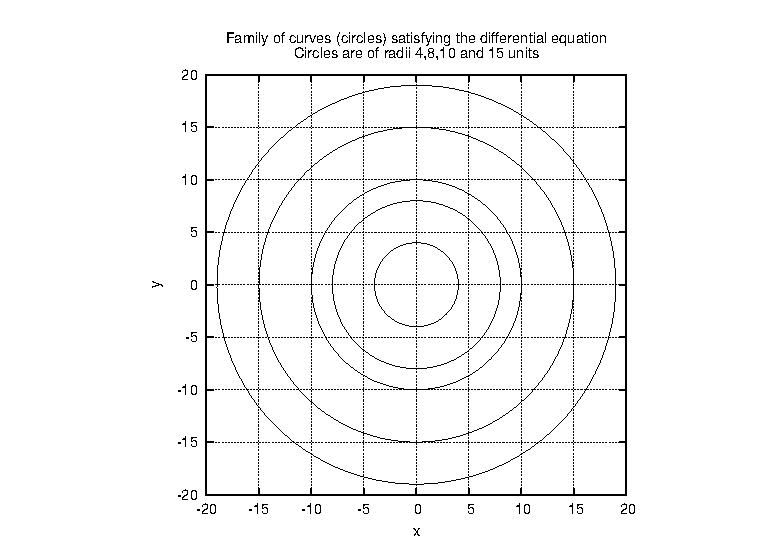
\includegraphics{circ}
\end{figure}
\textbf{Particular Solution}:
Substituting the given values y=10 when x=0, in $x^2+y^2=C$,
\[ 100 + 0 = C\]
\[C = 100\]
Hence, the particular solution is:
{\renewcommand{\arraystretch}{1.5}
\begin{tabular}{|c|}
\hline
$x^2 + y^2 = 100$\\
\hline
\end{tabular}}\\

\maketitle
3. The number of bacteria \emph{N} is 10,000 at time \emph{t}=0. At \emph{t}=3 hours, \emph{N}=500,000. Find the value of
\begin{enumerate}
\item[(i)]\emph{N} at \emph{t}=24 hours
\\
\item[(ii)]\emph{t} when \emph{N} is 20,000
\end{enumerate}
\emph{Answer}:
From theory, we know that the rate of change of the number of bacteria at a given time is proportional to the number of bacteria present at the time.
Thus,
\[ \frac{dN}{dt} = kN\]
Separating variables, we obtain:
\[ \frac{dN}{N} = kdt \]
Integrating, we obtain:
\[ lnN = kt + C_1\]
Simplifying,
\[N=k_1 e^{kt}\]
At time t=0, we have N=10000. Hence,
\[k_1 = 10000\]
Thus,
\[N=10000e^{kt}\]
At time t=3, we have N=500000,
Thus,
\[500000 = 10000 e^{k*3}\]
Thus,
\[k=\frac{1}{3}* ln50\]
\[k=1.304\]
\[N=100000e^{1.304t}\]

For (i),
\[N=10000*e^{1.304*24}\]
\begin{center}
{\renewcommand{\arraystretch}{1.5}
\begin{tabular}{|c|}
\hline
N=390553114652259072.000000\\
\hline
\end{tabular}}
\end{center}

For (ii), N=20000
\[20000 = 10000 * e^{1.304*t}\]
\[1.304*t = ln2\]
\begin{center}
\begin{tabular}{|c|}
\hline
t=0.903864 hours\\
\hline
\end{tabular}
\end{center}

\maketitle
3. $C_{14}$ isotope has a half-life of 5600 hours. What is the fraction that remains after 10,000 years?
\\
\emph{Answer}:
The mass of $C_{14}$ remaining after time \emph{t} can be modelled by the equation:
\[M=M_0e^{-kt}\]
where $M_0$ is the mass at time \emph{t}=0 and \emph{k} is a constant.
We are given data that the mass at \emph{t}=5600 years is half of the mass present initially.
Hence,
\[\frac{M_0}{2} = M_0e^{-5600k}\]
\[k=\frac{ln2}{5600}\]
\[k=0.000124\]
Thus,
\[M=M_0e^{-0.000124t}\]
At t=10000 years,
\[M=M_0e^{-1.24}\]
\[M=M_0*0.289384\]
Thus, the fraction remaining after 10000 years is \underline{0.289384}.
\end{document}
